\documentclass[11pt,a4paper]{article}
\usepackage[utf8]{inputenc}
\usepackage[hyperref]{emnlp2020}
\usepackage{times}
\usepackage{latexsym}
\usepackage{graphicx}
\usepackage{booktabs}
\usepackage{multirow}
\usepackage{amssymb,amsmath}
\renewcommand{\UrlFont}{\ttfamily\small}
\usepackage{caption}
\usepackage{subcaption}
\usepackage{fixltx2e}
\usepackage{soul}
\usepackage{siunitx}
\usepackage{microtype}
\usepackage{xcolor}
\usepackage{tablefootnote}
\usepackage{ulem}
\normalem

    \usepackage{tikz}
\usetikzlibrary{shapes}
\usetikzlibrary{arrows}
\usetikzlibrary{positioning}

\makeatletter
\DeclareRobustCommand*\textsubscript[1]{%
      \@textsubscript{\selectfont#1}}
      \def\@textsubscript#1{%
            {\m@th\ensuremath{_{\mbox{\fontsize\sf@size\z@#1}}}}}
            \makeatother

\usepackage[most]{tcolorbox}

\def\Snospace~{\S{}}
\renewcommand*\sectionautorefname{\Snospace}

\let\subsectionautorefname\sectionautorefname
\let\subsubsectionautorefname\sectionautorefname

\aclfinalcopy 
\def\aclpaperid{2916} 

\title{Controllable Meaning Representation to Text Generation: ~~~~
Linearization and Data Augmentation Strategies}

\author{Chris Kedzie \\
  Columbia University \\
  Department of Computer Science \\
  \texttt{kedzie@cs.columbia.edu} \\\And
  Kathleen McKeown \\
  Columbia University \\
  Department of Computer Science \\
  \texttt{kathy@cs.columbia.edu} \\}

\date{}

\begin{document} 
\maketitle 
\begin{abstract} 
    We study the degree to which sequence-to-sequence models exhibit fine-grained
controllability when performing natural language generation from a meaning
representation.  Using two task-oriented dialogue generation benchmarks, we
systematically compare the effect of four input linearization strategies on
controllability and faithfulness.  Additionally, we evaluate how a
phrase-based data augmentation method can improve performance.  We find that
properly aligning input sequences during training leads to highly controllable
generation on a variety of popular model architectures, both when training
from scratch or when fine-tuning a larger pre-trained model.  Phrase-based
data augmentation further improves control on difficult, randomly generated
utterance plans.

\end{abstract}

\newcommand{\placeholder}[1]{{\color{red}#1}}

\newcommand{\DA}[1]{\textsc{#1}}
\newcommand{\MR}[1]{\left[\!\!\!\left[ #1 \right]\!\!\!\right]}
\newcommand{\AV}[2]{\textrm{\textit{#1} = ``#2''}}
\newcommand{\Atr}[1]{\textit{#1}}
\newcommand{\Val}[1]{{``#1''}}
\newcommand{\U}[1]{\textit{#1}}

\newcommand{\mr}{\ensuremath{\mu}}
\newcommand{\MRs}{\ensuremath{\mathcal{M}}}
\newcommand{\attr}{\ensuremath{x}}
\newcommand{\utt}{\ensuremath{\mathbf{y}}}
\newcommand{\utttok}{\ensuremath{y}}

\newcommand{\Utts}{\ensuremath{\mathcal{Y}}}
\newcommand{\da}{\ensuremath{a}}
\newcommand{\mrSize}{m}

\newcommand{\lin}{\ensuremath{\pi}}
\newcommand{\Lins}{\ensuremath{\Pi}}

\newcommand{\Attrs}{\ensuremath{\mathcal{V}}}
\newcommand{\uttVocab}{\ensuremath{\mathcal{W}}}
\newcommand{\size}[1]{\ensuremath{{\lvert #1 \rvert}}}
\newcommand{\model}{\ensuremath{p}}

\newcommand{\lsname}[1]{\textit{#1}}
\newcommand{\lsshort}[1]{\textsc{#1}}

\newcommand{\bleu}{\textsc{Bleu}}
\newcommand{\rouge}{\textsc{Rouge}}
\newcommand{\rougel}{\textsc{Rouge-L}}

\newcommand{\phraseAug}{\textsc{+p}}


\newcommand{\biGRU}{biGRU}
\newcommand{\Transformer}{Transformer}
\newcommand{\BART}{BART}
\newcommand{\BgUP}{\textsc{BgUP}}
\newcommand{\NUP}{\textsc{NUP}}
\newcommand{\Oracle}{\textsc{Oracle}}

\newcommand{\lidstone}{\alpha}






%?\newcommand{\alignshort}{\lsshort{At}}
%?\newcommand{\LMRs}{\ensuremath{\mathcal{S}^{*}}}
%?\newcommand{\enc}{\ensuremath{f}}
%?\newcommand{\dec}{\ensuremath{g}}
%?\newcommand{\rep}{\ensuremath{h}}
%?\newcommand{\Reps}{\ensuremath{\mathcal{H}}}
%?
%?\newcommand{\inform}{\dastr{Inform}}
%?\newcommand{\genres}{\textit{genres}}
%?\newcommand{\eattype}{\textit{eat\_type}}
%?\newcommand{\area}{\textit{area}}
%?
\newcommand{\acount}{\ensuremath{\operatorname{count}}}
%?
%?\makeatletter
%?\newcommand{\MR}[1]{%
%?    $ \left[ \begin{array}{l} #1\checknextarg}
%?\newcommand{\checknextarg}{\@ifnextchar\bgroup{\gobblenextarg}{  \end{array}\right]$ }}
%?\newcommand{\gobblenextarg}[1]{ \\ #1\@ifnextchar\bgroup{\gobblenextarg}{ \end{array}\right]$ }}
%?
%?




\newcommand{\fencgruparams}[1]{\hat{\eta}^{(#1)}}
\newcommand{\rencgruparams}[1]{\check{\eta}^{(#1)}}
\newcommand{\decgruparams}[1]{{\zeta}^{(#1)}}
\newcommand{\embDim}{{D_w}}
\newcommand{\hidDim}{{D_h}}
\newcommand{\encEmbs}{\mathbf{E}}
\newcommand{\decEmbs}{\mathbf{D}}
\newcommand{\reals}{\mathbb{R}}
\newcommand{\encWordEmb}{\mathbf{v}} 
\newcommand{\decWordEmb}{\mathbf{w}} 
\newcommand{\inSize}{m}
\newcommand{\outSize}{n}
\newcommand{\inseq}{\mathbf{x}}
\newcommand{\zeroEmb}{\mathbf{0}}
\newcommand{\hstate}{\boldsymbol{h}}
\newcommand{\fhstate}{\boldsymbol{\hat{h}}}
\newcommand{\rhstate}{\boldsymbol{\check{h}}}
\newcommand{\fgru}{\operatorname{GRU}}
\newcommand{\gstate}{\boldsymbol{g}}
\newcommand{\astate}{\boldsymbol{\bar{h}}}
\newcommand{\fgstate}{\boldsymbol{\hat{g}}}
\newcommand{\rgstate}{\boldsymbol{\check{g}}}
\newcommand{\weight}[1]{\mathbf{W}^{(#1)}}
\newcommand{\bias}[1]{\mathbf{b}^{(#1)}}
\newcommand{\attnweight}{\mathbf{K}}
\newcommand{\attnvec}{\mathbf{k}}
\newcommand{\zstate}{\mathbf{z}}

\newcommand{\layerNorm}{\operatorname{LN}}
\newcommand{\mmhAttn}{\operatorname{maskedMHAttn}}
\newcommand{\mhAttn}{\operatorname{MHAttn}}
\newcommand{\MultiAttn}{\operatorname{MultiAttn}}
\newcommand{\Attn}{\operatorname{Attn}}
\newcommand{\softmax}{\operatorname{softmax}}
\newcommand{\feedforward}{\operatorname{FF}}
\newcommand{\relu}{\operatorname{ReLU}}

\newcommand{\Query}{\mathbf{Q}}
\newcommand{\Key}{\mathbf{K}}
\newcommand{\mrEmb}{\mathbf{W}}
\newcommand{\uttEmb}{\mathbf{V}}
\newcommand{\posEmb}{\mathbf{P}}
\newcommand{\encInput}{\mathbf{H}}
\newcommand{\decInput}{\mathbf{G}}
\newcommand{\decInputi}{\mathbf{g}_i}
\newcommand{\lnweight}{\mathbf{A}}
\newcommand{\lnweightv}{\mathbf{a}}
\newcommand{\lnbias}{\mathbf{b}}
\newcommand{\Mask}{\mathbf{M}}


\newcommand{\tfeA}{\boldsymbol{\check{\encInput}}^{(i)}}
\newcommand{\tfeB}{\boldsymbol{\bar{\encInput}}^{(i)}}
\newcommand{\tfeC}{\boldsymbol{\hat{\encInput}}^{(i)}}
\newcommand{\tfeD}{\boldsymbol{\dot{\encInput}}^{(i)}}
\newcommand{\tfeE}{\boldsymbol{\ddot{\encInput}}^{(i)}}

\newcommand{\tfdA}{\boldsymbol{\check{\decInput}}^{(i)}}
\newcommand{\tfdB}{\boldsymbol{\bar{\decInput}}^{(i)}}
\newcommand{\tfdC}{\boldsymbol{\hat{\decInput}}^{(i)}}
\newcommand{\tfdD}{\boldsymbol{\grave{\decInput}}^{(i)}}
\newcommand{\tfdE}{\boldsymbol{\tilde{\decInput}}^{(i)}}
\newcommand{\tfdF}{\boldsymbol{\acute{\decInput}}^{(i)}}
\newcommand{\tfdG}{\boldsymbol{\dot{\decInput}}^{(i)}}
\newcommand{\tfdH}{\boldsymbol{\ddot{\decInput}}^{(i)}}



\section{Introduction}

In this work, we study the degree to which neural sequence-to-sequence (S2S)
models exhibit fine-grained controllability when performing natural language
generation (NLG) from a meaning representation (MR).  In particular, we focus
on an  S2S approach that respects the realization ordering constraints of a
given utterance plan; such a model can generate utterances whose phrases
follow the order of the provided plan.
%phrase orderings 
%as indicated by
%the utterance plan. 

In non-neural NLG, fine-grained control for planning sentence structure has
received extensive study under the names \textit{sentence} or
\textit{micro-planning} \cite{reiter2000,walker2001,stone2003}.  Contemporary
practice, however, eschews modeling at this granularity, instead preferring to
train an S2S model to directly map an input MR to a natural language
utterance, with the utterance plan determined implicitly by the model
which is learned from the training data \cite{dusek2020}.
%the patterns
%exhibited in the training data and the model's decoder \cite{dusek2020}. 

We argue that robust and fine grained control in an S2S model is desirable
because it enables neural implementations of various psycho-linguistic
theories of discourse (e.g., Centering Theory \cite{grosz1995}, or
Accessibility Theory \cite{ariel2001}).  This could, in turn, encourage the
validation and/or refinement of additional psychologically plausible models of
language production.
 
\begin{figure}

{

    \begin{subfigure}{0.5\textwidth}
        \caption{\large~\textbf{E2E MR/Utterance Pair}}
    \end{subfigure}


    \centering
    \begin{subfigure}{0.25\textwidth}
         $\MR{\begin{array}{l}  
            \DA{Inform} \\
            \textrm{\footnotesize food = ``fast food''\textsuperscript{(1)}} \\
            \textrm{\footnotesize price = ``moderate''\textsuperscript{(2)}} \\
            \textrm{\footnotesize name = ``The Punter''\textsuperscript{(3)}}\\
        \end{array}}$
    \end{subfigure}\hfill\begin{subfigure}{0.19\textwidth}
        \textit{\ul{The Punter}\textsuperscript{3} is a 
            \ul{fast food}\textsuperscript{1} joint that is 
            \ul{not too expensive.}\textsuperscript{2}}
    \end{subfigure}
}

~\\



{
    \begin{subfigure}{0.5\textwidth}
        \caption{\large~\textbf{ViGGO MR/Utterance Pair}}
        \label{fig:exviggo}
    \end{subfigure}

    \centering
    \begin{subfigure}{0.25\textwidth}
        $\MR{\begin{array}{l}  
            \DA{Request} \\ 
            \DA{Explanation} \\
            \textrm{\footnotesize genres = [}\\
            \textrm{\footnotesize~~~~``role-playing'',\textsuperscript{(1)}} \\
            \textrm{\footnotesize~~~~``hack-and-slash'',\textsuperscript{(2)}]} \\
            \textrm{\footnotesize ESRB = ``M (Mature)''\textsuperscript{(3)}}\\
            \textrm{\footnotesize rating = ``good''\textsuperscript{(4)}} \\ 
        \end{array}}$

    \end{subfigure}\hfill\begin{subfigure}{0.19\textwidth}
        \textit{What is it about \ul{M rated}\textsuperscript{3} 
            \ul{hack-and-slash}\textsuperscript{2} \ul{RPGs}\textsuperscript{1}
            that \ul{makes you enjoy them?}\textsuperscript{4}}
    \end{subfigure}
}

\caption{(a) Example MR for \DA{Inform} dialogue act (left) and utterance
    (right) pair from the E2E dataset. (b) Example MR for \DA{Request
    Explanation} dialogue act (left) and utterance (right) pair from the ViGGO
    dataset. Superscripts indicate which attribute-values correspond to which
    utterance sub-spans.}
\label{fig:examples}
\end{figure}


In this paper, we study controllability in the context of task-oriented
dialogue generation \cite{mairesse2010,wen2015}, where the input to the NLG
model is an MR consisting of a dialogue act (i.e. a communicative goal) such as
to \DA{Request Explanation}, and an unordered set of attribute-value pairs
defining the semantics of the intended utterance (see \autoref{fig:examples}
for an example). 


The NLG model is expected to produce an utterance that adequately and
faithfully communicates the MR.  In the S2S paradigm, the MR must be
``linearized'' (i.e.  represented as a linear sequence of tokens corresponding
to the dialogue act and attribute-value pairs) before being presented to the S2S
 encoder.  We explore several linearization strategies and measure
their effectiveness for controlling phrase order, as well as their effect on
 model faithfulness (i.e., the semantic correctness of generated utterances).

 Of particular note, \textit{alignment training} (i.e.  at training time, linearizing
the attribute-value pairs according to the order in which they are realized by
their corresponding reference utterance) produces highly controllable  S2S
models.  While we are not the first to observe this (c.f., \citet{nayak2017}),
we study this behavior extensively.  We refer to an ordered sequence of
attribute-value pairs $\attr_1, \attr_2, \ldots, \attr_n$ as an
\textit{utterance plan}, and evaluate models on their ability to follow such
plans given by either another model, a human, or, most difficultly, from
random permutation.

Additionally, we experiment with a data augmentation method, where we create
fragmentary MR/utterance pairs obtained from the constituent phrases of the
original training data.  We find that this data augmentation results in
reduced semantic error rates and increases the ability of a model to follow an
arbitrary utterance plan.

 We summarize our contributions as follows. (1) We show that \textbf{alignment training
produces highly controllable %and faithful 
language generation models},
%in both recurrent and non-recurrent S2S models, 
especially when following a model created utterance plan. (2) We demonstrate that \textbf{phrase-based
data augmentation improves the robustness of the control} even on arbitrary
and difficult to follow utterance plans. (3) We conclude with a human
evaluation that shows that \textbf{phrase-based data augmentation training
can increase the robustness of control without hurting fluency.}\footnote{
    Code, outputs, augmented data, and other materials 
    can be found here: \url{https://github.com/kedz/cmr2text}.}




\section{Methods}

In an MR-to-text task, we are given as input an MR $\mr \in \MRs$ from which
to generate an appropriate natural language utterance $\utt  \in \Utts$, where
\mr~consists of a dialogue act that characterizes the communicative goal of the
utterance and an unordered and variably sized set of attribute-value pairs.
Attributes are either binary or categorical variables (e.g.,
\Atr{family-friendly}: [``yes'', ``no''] or \Atr{food}: [``Chinese'',
``English'', ``French'', $\ldots$]).\footnote{There are also list-valued
attributes but we treat them as individual attribute-value pairs (i.e. in
\autoref{fig:examples}, both \AV{genres}{role-playing} and
\AV{genres}{hack-and-slash} are in $\mr$).}

Let each attribute-value pair \attr~and dialogue act \da~be tokens from a
vocabulary \Attrs, and define the size of an MR, denoted  $\size{\mr}$,  to be
the number of attribute-values $\attr \in \mr$.  A linearization
strategy $\lin : \MRs \rightarrow \Attrs^*$ is a mapping of the dialogue act
and attribute-values in \mr~to an ordered sequence, i.e.  $\lin(\mr) = [\da,
\attr_1, \attr_2, \ldots, \attr_\size{\mr}]$.  Regardless of the choice of
\lin, the first token in $\lin(\mr)$ is always the dialogue act \da.

We experiment with both gated recurrent unit (GRU) \cite{cho2014} and
Transformer \cite{vaswani2017} based S2S model variants to implement a
conditional probability model $\model(\cdot| \lin(\mr); \theta) : \Utts
\rightarrow (0, 1)$ over utterances. The model parameters,
$\theta$ are learned by approximately maximizing the log-likelihood
$\mathcal{L}(\theta)= \sum_{(\mr,\utt)\in \mathcal{D}}  \log
\model(\utt|\lin(\mr); \theta)$ on the training set $\mathcal{D}$.
Additionally, we experiment with a pretrained S2S Transformer, BART
\cite{lewis2020}, with parameters $\theta_0$ fine-tuned on
$\mathcal{L}(\theta_0)$.

\subsection{Linearization Strategies}
\label{sec:linstrats}

Because of the recurrence in the GRU and position embeddings in the
Transformer, it is usually the case that different linearization
strategies, i.e.  $\lin(\mr) \ne \lin^\prime(\mr)$, will result in different
model internal representations and therefore different conditional probability
distributions. These differences can be non-trivial, yielding changes in model
behavior with respect to faithfulness and control.

We study four linearization strategies, \lsname{(i) random}, \lsname{(ii)
increasing-frequency}, \lsname{(iii) fixed-position}, and \lsname{(iv)
alignment training}, which we describe below. For visual examples of each
strategy, see \autoref{fig:linstrats}.  Note that linearization determines the
order of the attribute-value pairs presented to the S2S encoder, and \textbf{only} in the
case of alignment training does it correspond to the order in which the
attribute-value pairs are realized in the utterance. When presenting a linearized
MR to the model encoder, we always prepend and append distinguished
\textit{start} and \textit{stop} tokens respectively.


\newtcbox{\mybox}[1][]{enhanced, colframe=blue, colback=blue!15, 
                       nobeforeafter, tcbox raise base, shrink tight, extrude 
                       by=0.75mm, #1}



\begin{figure*}
    \center
    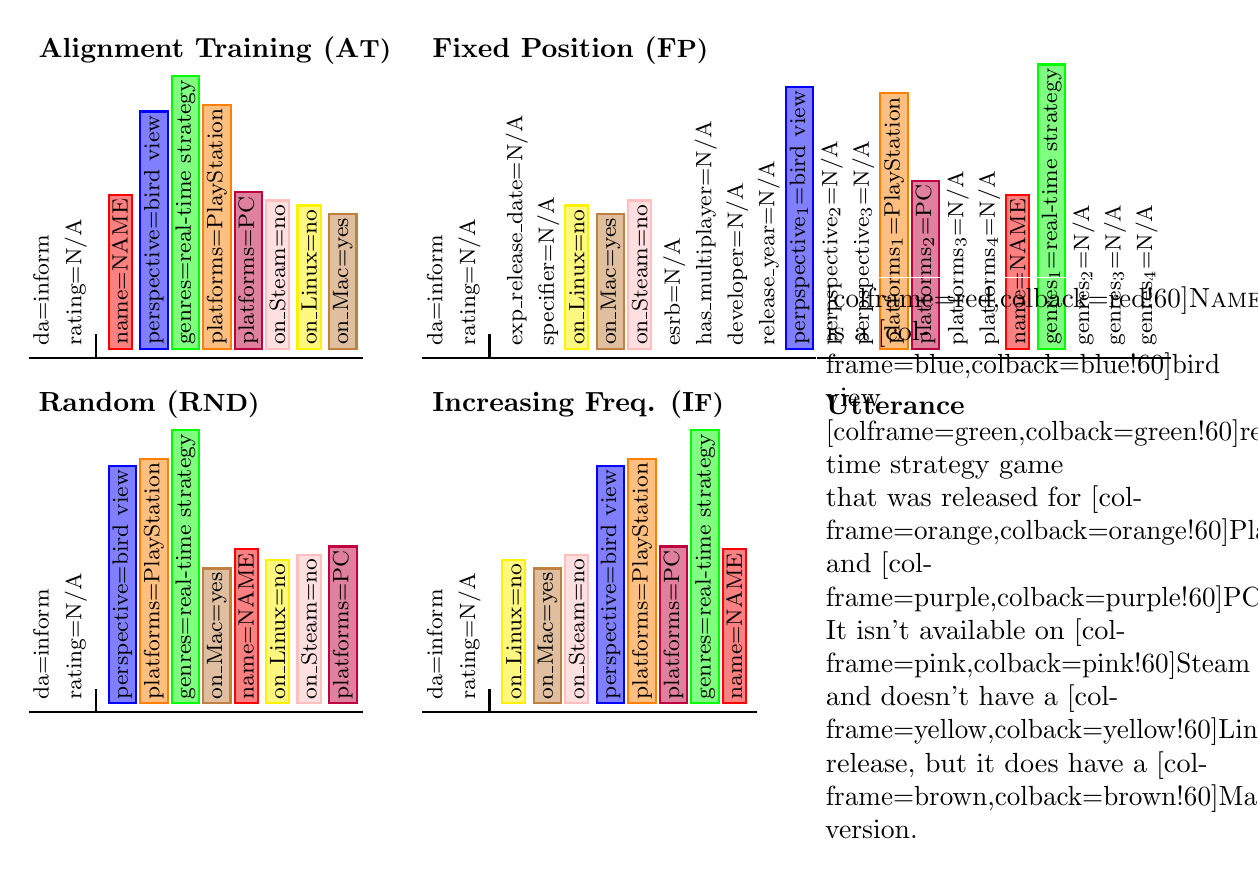
\begin{tikzpicture}[]


    \node[anchor=west] at (5.0,5.8) 
        {\textbf{Fixed Position \textsc{(F\small{P})}}};
    \node[anchor=west] at (0.0,5.8) 
        {\textbf{Alignment Training \textsc{(A\small{T})}}};
    \draw[thick] (0.85,1.9) -- (0.85,2.2);
    \draw[thick] (0,1.9) -- (4.25,1.9);
    \draw[thick] (5 + 0.85,1.9) -- (5 + 0.85,2.2);
    \draw[thick] (5 + 0,1.9) -- (10.25+ 4.25,1.9);
    \draw[thick] (0.85,-2.6) -- (0.85,-2.3);
    \draw[thick] (0,-2.6) -- (4.25,-2.6);
    \draw[thick] (5+0.85,-2.6) -- (5+0.85,-2.3);
    \draw[thick] (5+0,-2.6) -- (5+4.25,-2.6);

    \node[anchor=north west,inner sep=0.5mm,rotate=90] at (0,2) 
        {\footnotesize da=inform};
    \node[anchor=north west,inner sep=0.5mm,rotate=90] at (0.4,2) 
        {\footnotesize rating=N/A};
    \node[anchor=north west,rotate=90,inner sep=0.5mm,draw=red,thick,fill=red!50] 
        at (0.2 + 0.8,2) 
        {\footnotesize name=NAME};
    \node[anchor=north west,rotate=90,inner sep=0.5mm,draw=blue,thick,fill=blue!50] 
        at (0.2 + 1.2,2) {\footnotesize perspective=bird view};
    \node[anchor=north west,rotate=90,inner sep=0.5mm,draw=green,thick,
          fill=green!50] 
        at (0.2 + 1.6,2) {\footnotesize genres=real-time strategy};
    \node[anchor=north west,rotate=90,inner sep=0.5mm,draw=orange,thick,
          fill=orange!50] 
        at (0.2 + 2.0,2) {\footnotesize platforms=PlayStation};
    \node[anchor=north west,rotate=90,inner sep=0.5mm,draw=purple,thick,
          fill=purple!50] 
        at (0.2 + 2.4,2) {\footnotesize platforms=PC};
    \node[anchor=north west,rotate=90,inner sep=0.5mm,draw=pink,thick,
          fill=pink!50] 
        at (0.2 + 2.8,2) {\footnotesize on\_Steam=no};
    \node[anchor=north west,rotate=90,inner sep=0.5mm,draw=yellow,thick,
          fill=yellow!50] 
        at (0.2 + 3.2,2) {\footnotesize on\_Linux=no};
    \node[anchor=north west,rotate=90,inner sep=0.5mm,draw=brown,thick,
          fill=brown!50] 
        at (0.2 + 3.6,2) {\footnotesize on\_Mac=yes};


\node[anchor=north west,inner sep=0.5mm,rotate=90] at (5 + 0,2) 
    {\footnotesize da=inform};
\node[anchor=north west,inner sep=0.5mm,rotate=90] at (5 + 0.4,2) 
    {\footnotesize rating=N/A};
\node[anchor=north west,rotate=90,inner sep=0.5mm] 
    at (5.2 + 0.8,2) 
    {\footnotesize exp\_release\_date=N/A};
\node[anchor=north west,rotate=90,inner sep=0.5mm] 
    at (5.2 + 1.2,2) 
    {\footnotesize specifier=N/A};
\node[anchor=north west,rotate=90,inner sep=0.5mm,draw=yellow,thick,fill=yellow!50] 
    at (5.2 + 1.6,2) 
    {\footnotesize on\_Linux=no};
\node[anchor=north west,rotate=90,inner sep=0.5mm,draw=brown,thick,fill=brown!50] 
    at (5.2 + 2.0,2) 
    {\footnotesize on\_Mac=yes};
\node[anchor=north west,rotate=90,inner sep=0.5mm,draw=pink,thick,fill=pink!50] 
    at (5.2 + 2.4,2) 
    {\footnotesize on\_Steam=no};
\node[anchor=north west,rotate=90,inner sep=0.5mm] 
    at (5.2 + 2.8,2) 
    {\footnotesize esrb=N/A};
\node[anchor=north west,rotate=90,inner sep=0.5mm] 
    at (5.2 + 3.2,2) 
    {\footnotesize has\_multiplayer=N/A};

   % ['inform', 'rating=N/A', 'exp_release_date=N/A', 'specifier=N/A', 'has_linux_release=no', 'has_mac_release=yes', 'available_on_steam=no', 'esrb=N/A', 'has_multiplayer=N/A', 'developer=N/A', 'release_year=N/A', 'player_perspective=bird view', 'player_perspective=N/A', 'player_perspective=N/A', 'platforms=PlayStation', 'platforms=PC', 'platforms=N/A', 'platforms=N/A', 'name=PLACEHOLDER', 'genres=real-time strategy', 'genres=N/A', 'genres=N/A', 'genres=N/A']
\node[anchor=north west,rotate=90,inner sep=0.5mm] 
    at (5.2 + 3.6,2) 
    {\footnotesize developer=N/A};
\node[anchor=north west,rotate=90,inner sep=0.5mm] 
    at (5.2 + 4.0,2) 
    {\footnotesize release\_year=N/A};
\node[anchor=north west,rotate=90,inner sep=0.5mm,draw=blue,thick,fill=blue!50] 
    at (5.2 + 4.4,2) 
    {\footnotesize perpspective\textsubscript{1}=bird view};
\node[anchor=north west,rotate=90,inner sep=0.5mm] 
    at (5.2 + 4.8,2) 
    {\footnotesize perpspective\textsubscript{2}=N/A};
\node[anchor=north west,rotate=90,inner sep=0.5mm] 
    at (5.2 + 5.2,2) 
    {\footnotesize perpspective\textsubscript{3}=N/A};
\node[anchor=north west,rotate=90,inner sep=0.5mm,draw=orange,thick,fill=orange!50] 
    at (5.2 + 5.6,2) 
    {\footnotesize platforms\textsubscript{1}=PlayStation};
\node[anchor=north west,rotate=90,inner sep=0.5mm,draw=purple,thick,fill=purple!50] 
    at (5.2 + 6.0,2) 
    {\footnotesize platforms\textsubscript{2}=PC};
\node[anchor=north west,rotate=90,inner sep=0.5mm] 
    at (5.2 + 6.4,2) 
    {\footnotesize platforms\textsubscript{3}=N/A};
\node[anchor=north west,rotate=90,inner sep=0.5mm] 
    at (5.2 + 6.8,2) 
    {\footnotesize platforms\textsubscript{4}=N/A};
\node[anchor=north west,rotate=90,inner sep=0.5mm,draw=red,thick,fill=red!50] 
    at (5.2 + 7.2,2) 
    {\footnotesize name=NAME};
\node[anchor=north west,rotate=90,inner sep=0.5mm,draw=green,thick,fill=green!50] 
    at (5.2 + 7.6,2) 
    {\footnotesize genres\textsubscript{1}=real-time strategy};
\node[anchor=north west,rotate=90,inner sep=0.5mm] 
    at (5.2 + 8.0,2) 
    {\footnotesize genres\textsubscript{2}=N/A};
\node[anchor=north west,rotate=90,inner sep=0.5mm] 
    at (5.2 + 8.4,2) 
    {\footnotesize genres\textsubscript{3}=N/A};
\node[anchor=north west,rotate=90,inner sep=0.5mm] 
    at (5.2 + 8.8,2) 
    {\footnotesize genres\textsubscript{4}=N/A};


%\node[anchor=north west,rotate=90] at (1.5,2) {genres=platformer};
%\node[anchor=north west,rotate=90] at (2,2) {genres=puzzle};
%\node[anchor=north west,rotate=90] at (2.5,2) {perspective=side vew};
%\node[anchor=north west,rotate=90] at (3,2) {name=NAME};
%\node[anchor=north west,rotate=90] at (3.5,2) {name=NAME};
%\node[anchor=north west,rotate=90] at (4,2) {name=NAME};
%\node[anchor=north west,rotate=90] at (4.5,2) {name=NAME};
%
%
%\node[anchor=north west,rotate=90] at (5.5+0,2) {\small give opinion};
%\node[anchor=north west,rotate=90] at (5.5+0.5,2) {\small rating=good};
%\node[anchor=north west,rotate=90] at (5.5+1,2) {\small genres=adventure};
%\node[anchor=north west,rotate=90] at (5.5+1.5,2) {genres=platformer};
%\node[anchor=north west,rotate=90] at (5.5+2,2) {genres=puzzle};
%\node[anchor=north west,rotate=90] at (5.5+2.5,2) {perspective=side vew};
%\node[anchor=north west,rotate=90] at (5.5+3,2) {name=NAME};
%\node[anchor=north west,rotate=90] at (5.5+3.5,2) {name=NAME};
%\node[anchor=north west,rotate=90] at (5.5+4,2) {name=NAME};
%\node[anchor=north west,rotate=90] at (10+0,2) {give opinion};
%\node[anchor=north west,rotate=90] at (10+0.5,2) {rating=good};
%\node[anchor=north west,rotate=90] at (10+1,2) {genres=adventure};
%\node[anchor=north west,rotate=90] at (10+1.5,2) {genres=platformer};
%\node[anchor=north west,rotate=90] at (10+2,2) {genres=puzzle};
%\node[anchor=north west,rotate=90] at (10+2.5,2) {perspective=side vew};
%\node[anchor=north west,rotate=90] at (10+3,2) {name=NAME};
%\node[anchor=north west,rotate=90] at (10+3.5,2) {name=NAME};
%\node[anchor=north west,rotate=90] at (10+4,2) {name=NAME};
%\node[anchor=north west,rotate=90] at (10+4.5,2) {name=NAME};
%
%



%['give_opinion', 'rating=good', 'genres=adventure', 'genres=platformer', 'genres=puzzle', 'player_perspective=side view', 'name=PLACEHOLDER']


%#
%#

%['inform', 'rating=N/A', 'exp_release_date=N/A', 'specifier=N/A', 'has_linux_release=no', 'has_mac_release=yes', 'available_on_steam=no', 'esrb=N/A', 'has_multiplayer=N/A', 'developer=N/A', 'release_year=N/A', 'player_perspective=bird view', 'player_perspective=N/A', 'player_perspective=N/A', 'platforms=PlayStation', 'platforms=PC', 'platforms=N/A', 'platforms=N/A', 'name=PLACEHOLDER', 'genres=real-time strategy', 'genres=N/A', 'genres=N/A', 'genres=N/A']


%inc_freq_delex
%['inform', 'rating=N/A', 'has_linux_release=no', 'has_mac_release=yes', 'available_on_steam=no', 'player_perspective=bird view', 'platforms=PlayStation', 'platforms=PC', 'name=PLACEHOLDER', 'genres=real-time strategy']

\node[anchor=north west,inner sep=0.5mm,rotate=90] at (0,-2.5) 
    {\footnotesize da=inform};
\node[anchor=north west,inner sep=0.5mm,rotate=90] at (0.4,-2.5) 
    {\footnotesize rating=N/A};
\node[anchor=north west,rotate=90,inner sep=0.5mm,draw=blue,thick,fill=blue!50] 
    at (0.2 + 0.8,-2.5) 
    {\footnotesize perspective=bird view};

\node[anchor=north west,rotate=90,inner sep=0.5mm,draw=orange,thick,fill=orange!50] 
    at (0.2 + 1.2,-2.5) 
    {\footnotesize platforms=PlayStation};
\node[anchor=north west,rotate=90,inner sep=0.5mm,draw=green,thick,fill=green!50] 
    at (0.2 + 1.6,-2.5) 
    {\footnotesize genres=real-time strategy};


\node[anchor=north west,rotate=90,inner sep=0.5mm,draw=brown,thick,fill=brown!50] 
    at (0.2 + 2.0,-2.5) 
    {\footnotesize on\_Mac=yes};
\node[anchor=north west,rotate=90,inner sep=0.5mm,draw=red,thick,fill=red!50] 
    at (0.2 + 2.4,-2.5) 
    {\footnotesize name=NAME};

\node[anchor=north west,rotate=90,inner sep=0.5mm,draw=yellow,thick,fill=yellow!50] 
    at (0.2 + 2.8,-2.5) 
    {\footnotesize on\_Linux=no};
\node[anchor=north west,rotate=90,inner sep=0.5mm,draw=pink,thick,fill=pink!50] 
    at (0.2 + 3.2,-2.5) 
    {\footnotesize on\_Steam=no};
\node[anchor=north west,rotate=90,inner sep=0.5mm,draw=purple,thick,fill=purple!50] 
    at (0.2 + 3.6,-2.5) 
    {\footnotesize platforms=PC};

    \node[anchor=west] at (0,1.3) {\textbf{Random \textsc{(R\small{ND})}}};



\node[anchor=north west,inner sep=0.5mm,rotate=90] at (5 + 0,-2.5) 
    {\footnotesize da=inform};
\node[anchor=north west,inner sep=0.5mm,rotate=90] at (5 + 0.4,-2.5) 
    {\footnotesize rating=N/A};
\node[anchor=north west,rotate=90,inner sep=0.5mm,draw=yellow,thick,fill=yellow!50] 
    at (5.2 + 0.8,-2.5) 
    {\footnotesize on\_Linux=no};
\node[anchor=north west,rotate=90,inner sep=0.5mm,draw=brown,thick,fill=brown!50] 
    at (5.2 + 1.2,-2.5) 
    {\footnotesize on\_Mac=yes};
\node[anchor=north west,rotate=90,inner sep=0.5mm,draw=pink,thick,fill=pink!50] 
    at (5.2 + 1.6,-2.5) 
    {\footnotesize on\_Steam=no};

\node[anchor=north west,rotate=90,inner sep=0.5mm,draw=blue,thick,fill=blue!50]
    at (5.2 + 2.0,-2.5) 
    {\footnotesize perspective=bird view};
\node[anchor=north west,rotate=90,inner sep=0.5mm,draw=orange,thick,fill=orange!50] 
    at (5.2 + 2.4,-2.5) 
    {\footnotesize platforms=PlayStation};
\node[anchor=north west,rotate=90,inner sep=0.5mm,draw=purple,thick,fill=purple!50] 
    at (5.2 + 2.8,-2.5) 
    {\footnotesize platforms=PC};

\node[anchor=north west,rotate=90,inner sep=0.5mm,draw=green,thick,fill=green!50] 
    at (5.2 + 3.2,-2.5) 
    {\footnotesize genres=real-time strategy};
\node[anchor=north west,rotate=90,inner sep=0.5mm,draw=red,thick,fill=red!50] 
    at (5.2 + 3.6,-2.5) 
    {\footnotesize name=NAME};
%has_linux_release=no', 'has_mac_release=yes', 'available_on_steam=no', 'player_perspective=bird view', 'platforms=PlayStation', 'platforms=PC', 'name=PLACEHOLDER', 'genres=real-time strategy'
    \node[anchor=west] at (5.0,1.3) {\textbf{Increasing Freq. \textsc{(I\small{F})}}};


%\node[anchor=north west,inner sep=0.5mm,rotate=90] at (10 + 0,-2.5) 
%    {\footnotesize da=inform};
%\node[anchor=north west,inner sep=0.5mm,rotate=90] at (10 + 0.4,-2.5) 
%    {\footnotesize rating=N/A};
%
%\node[anchor=north west,rotate=90,inner sep=0.5mm,draw=red,thick,fill=red!50] 
%    at (10.2 + 0.8,-2.5) 
%    {\footnotesize name=NAME};
%
%\node[anchor=north west,rotate=90,inner sep=0.5mm,draw=green,thick,fill=green!50] 
%    at (10.2 + 1.2,-2.5) 
%    {\footnotesize genres=real-time strategy};
%
%    \node[anchor=north west,rotate=90,inner sep=0.5mm,draw=purple,thick,fill=purple!50] 
%    at (10.2 + 1.6,-2.5) 
%    {\footnotesize platforms=PC};
%\node[anchor=north west,rotate=90,inner sep=0.5mm,draw=orange,thick,fill=orange!50] 
%    at (10.2 + 2.0,-2.5) 
%    {\footnotesize platforms=PlayStation};
%
%\node[anchor=north west,rotate=90,inner sep=0.5mm,draw=blue,thick,fill=blue!50]
%    at (10.2 + 2.4,-2.5) 
%    {\footnotesize perspective=bird view};
%\node[anchor=north west,rotate=90,inner sep=0.5mm,draw=pink,thick,fill=pink!50] 
%    at (10.2 + 2.8,-2.5) 
%    {\footnotesize on\_Steam=no};
%\node[anchor=north west,rotate=90,inner sep=0.5mm,draw=brown,thick,fill=brown!50] 
%    at (10.2 + 3.2,-2.5) 
%    {\footnotesize on\_Mac=yes};
%\node[anchor=north west,rotate=90,inner sep=0.5mm,draw=yellow,thick,fill=yellow!50] 
%    at (10.2 + 3.6,-2.5) 
%    {\footnotesize on\_Linux=no};
%




%has_linux_release=no', 'has_mac_release=yes', 'available_on_steam=no', 'player_perspective=bird view', 'platforms=PlayStation', 'platforms=PC', 'name=PLACEHOLDER', 'genres=real-time strategy'
%    \node[anchor=west] at (10.0,1.3) {\textbf{Decreasing Freq.}};




    \node[anchor=west] at (10, 1.3) {\textbf{Utterance}};
\node[text width=5.0cm,draw=white,anchor=west] at (10,-0.7) {
    {\mybox[colframe=red,colback=red!60]{\textsc{Name}}} is a 
    \mybox[colframe=blue,colback=blue!60]{bird view} 
    \mybox[colframe=green,colback=green!60]{real-time strategy} 
    game that was released for 
    \mybox[colframe=orange,colback=orange!60]{PlayStation} and 
    \mybox[colframe=purple,colback=purple!60]{PC.} It isn't available on 
    \mybox[colframe=pink,colback=pink!60]{Steam} and doesn't have a 
    \mybox[colframe=yellow,colback=yellow!60]{Linux} release, but it does have
    a \mybox[colframe=brown,colback=brown!60]{Mac} version.
};


\end{tikzpicture}

\caption{Example MR linearization strategies for the utterance above from the
    ViGGO training set.}
\label{fig:linstrats}
\end{figure*}


\paragraph{Random (\textsc{Rnd})} In the \lsname{random} linearization
(\lsshort{Rnd}), we randomly order the attribute-value pairs for a given MR.
This strategy serves as a baseline for determining if linearization 
matters at all for faithfulness. \lsshort{Rnd} is similar to token level noise
used in denoising auto-encoders \cite{wang2019} and might
even improve faithfulness.  During training, we resample the ordering for each
example at every epoch.  We do not resample the validation set in order to
obtain stable results for model selection.

\paragraph{Increasing Frequency (\textsc{If})} In the \lsname{increasing
frequency} linearization (\lsshort{If}), we order the attribute-value pairs by
increasing frequency of occurrence in the training data (i.e., $\acount(\attr_i)
\le \acount(\attr_{i+1})$).  We hypothesize that placing frequently occurring
items in a consistent location may make it easier for $\model$ to realize
those items correctly, possibly at the expense of rarer items.

\paragraph{Fixed Position (\textsc{Fp})} We take  consistency one step further
and create a fixed ordering of all attributes, \textit{n.b.} not
attribute-values, ordering them in increasing frequency of occurrence on the
training set (i.e. every instance has the same order of attributes in the
encoder input). In this \lsname{fixed position} linearization (\lsshort{Fp}),
attributes that are not present in an MR are explicitly represented with an
\Val{N/A} value.  For list-valued slots, we determine the maximum length
list in the training data and create that many repeated slots in the input
sequence.  This linearization is feasible for datasets with a modest number of
unique attributes %(in our case Viggo has 14 attributes and E2E eight) 
but may 
not easily scale to 10s, 100s, or larger attribute vocabularies. 

\paragraph{Alignment Training (\textsc{At})} 

In the \lsname{alignment training} linearization (\lsshort{At}), during
training, the order of attribute-value pairs $\attr_1, \attr_2, \ldots,
\attr_\size{\mr}$ matches the order in which they are realized in the
corresponding training utterance.  This is feasible because in the majority of
cases, there is a one-to-one mapping of attribute-values and utterance
subspans.

%%  %Training $\model$ with this strategy yields a model
%%  %that is highly controllable, i.e. when conditioning on $\lin(\mr) = [\da, \attr_i, \attr_{i+1}, \ldots]$, $\model(\cdot|\lin(\mr);\theta)$ will 
%%  %place higher probability on utterances where $\attr_i$ is realized first,
%%  %followed by $\attr_{i+1}$, and so on.

We obtain this ordering using a manually constructed set of matching rules to
identify which utterance subspans correspond to each attribute-value pair
(see \autoref{sec:align}).

Crucially, \lsshort{At}~stands in contrast to the  first three strategies
(\lsshort{Rnd}, \lsshort{If}, and \lsshort{Fp}) which do not have any
correspondence between the the order of attribute-value pairs in $\lin(\mr)$
and the order in which they are realized in the corresponding utterance
$\utt$. %and as a  result, models trained with those strategies %are not controllable. 
%KM - Again, isn't this something you will show through your experiments?




At test time, when there is no reference utterance \lsshort{At}
cannot specify a linearization. However, models trained with \lsshort{At}
can generate an  utterance from an arbitrary utterance plan
$\attr_1, \attr_2, \ldots, \attr_{\size{\mr}}$ 
provided by an external source, such as an utterance planner model or human 
reference. See \autoref{fig:ctrlouts} for an example of how an \lsshort{At}-trained model might follow three different plans for the same MR.
%%  %. We refer to such an ordering as an {\em utterance plan}.
%%  %KM - I put in italics. This sentence implies it's the first time mentioned, but you mention t in the intro. Perhaps you can define it there? 

\begin{figure}
    \resizebox{.48\textwidth}{!}{%
        \begin{tabular}{l}
            \toprule
            $\lin\left(\mr\right) = \left[\textrm{inform}, 
                \textrm{name=Aromi}, \textrm{eat\_type=coffee shop}, 
                \textrm{area=city centre} \right]$\\
            $\hat{\utt} = \textit{Aromi is a coffee shop in the city 
                centre.}$\\
            \midrule
            $\lin\left(\mr\right) = \left[\textrm{inform}, 
                \textrm{eat\_type=coffee shop}, \textrm{name=Aromi}, 
                \textrm{area=city centre} \right]$\\
            $\hat{\utt} = \textit{There is a coffee shop called Aromi in the 
                city centre.}$\\
            \midrule
            $\lin\left(\mr\right) = \left[\textrm{inform}, 
                \textrm{eat\_type=coffee shop}, \textrm{area=city centre}, 
                \textrm{name=Aromi} \right]$\\
            $\hat{\utt} = \textit{For coffee in the centre of the city, try 
                Aromi.}$\\
            \bottomrule
        \end{tabular}
    }
    \caption{Example outputs ($\hat{\utt}$) from a controllable model, 
i.e. a S2S model trained with \lsshort{At} linearization, 
under different input utterance plans ($\lin\left(\mr\right)$).}
\label{fig:ctrlouts}
\end{figure}


\begin{table}
\begin{tabular}{ccccc}
\toprule
            & \multicolumn{2}{c}{E2E} & \multicolumn{2}{c}{Viggo}\\
        \cmidrule(lr){2-3}
        \cmidrule(lr){4-5}
                & Orig. & Phr. & Orig. & Phr. \\
\midrule
\# ex. & 33,523 & 443,192 &  5,103  & 67,445 \\
Avg. $\size{\mr}$ &5.3 & 1.8 & 6.8 & 3.8\\
Avg. $\size{\utt}$ &23.6 & 7.0& 24.4 & 6.7\\
\bottomrule
\end{tabular}
\caption{Statistics of original training and phrase data.}
\label{tab:main.dataset.stats}
\end{table}

\subsection{Phrase-based Data Augmentation}

We augment the training data with MR/utterance pairs taken from constituent
phrases in the original training data.  We parse all training utterances and
enumerate all constituent phrases governed by NP, VP, ADJP, ADVP, PP, S, Sbar
non-terminals.\footnote{We used the
\href{https://stanfordnlp.github.io/CoreNLP/}{Stanford CoreNLP parser
v3.9.2}.} We then apply the attribute-value matching rules used for
\lsshort{At} (see \autoref{sec:align}) to obtain a corresponding MR, keeping
the dialog act of the original utterance. We discard phrases with no realized
attributes.  See \autoref{tab:main.dataset.stats} for augmented data
statistics.

Because we re-classify the MR of phrases using the matching rules, the
augmented  data includes examples of how to invert binary attributes, e.g.
from the phrase ``\U{is not on Mac,}'' which implies
\AV{has\_mac\_release}{no,} we obtain the phrase ``\U{on Mac}''
which implies \AV{has\_mac\_release}{yes.} When presenting the linearized
MR of phrase examples to the model encoder we prepend and append phrase
specific \textit{start} and \textit{stop} tokens respectively (e.g.,
\textit{start-NP} and \textit{stop-NP}) to discourage the model from ever
producing an incomplete sentence when generating for a complete MR.



\section{Datasets}

We run our experiments on two English language, task-oriented dialogue
datasets, the \href{http://www.macs.hw.ac.uk/InteractionLab/E2E/}{E2E
Challenge} corpus \cite{novikova2017} and the
\href{https://nlds.soe.ucsc.edu/viggo}{ViGGO} corpus \cite{juraska2019}. These
datasets provide MR/utterance pairs from the restaurant and video game
domains, respectively. Examples from the E2E corpus (33,523 train/1,426
dev/630 test) can have up to eight unique attributes.  There is only one
dialog act for the corpus, \DA{Inform}.  Attribute-values are either binary or
categorical valued.

The ViGGO corpus (5,103 train/246 dev/359 test) contains 14 attribute types
and nine dialog acts (\DA{Request Explanation}, \DA{Recommend}, etc.).  In
addition to binary and categorical valued attributes, the corpus also features
list-valued attributes (see the \Atr{genres} attribute in
\autoref{fig:exviggo}) which can have a variable number of values, and an
open-class \Atr{specifier} attribute. 

\subsection{MR/Utterance Alignments}
\label{sec:align}

The original datasets do not have alignments between individual
attribute-values and the subspans of the utterances they occur in, which we
need for the \lsshort{At} linearization strategy.  We manually developed a
list of heuristic pattern matching rules (e.g. \textit{not kid-friendly}
$\rightarrow$ \AV{family\_friendly}{no}).  For ViGGO, we started from
scratch, but for E2E we greatly expanded the rule-set created by
\citet{dusek2019}.  To ensure the correctness of the rules, we
iteratively added new matching rules, ran them on the training and validation
sets, and verified that they produced the same MR as was provided in the
dataset. This process took one author roughly two weeks to produce
approximately 25,000 and 1,500 rules for the E2E and ViGGO datasets
respectively. Note that the large number of rules is obtained
programmatically, i.e. creating template rules and inserting matching keywords
or phrases (e.g., enumerating variants such as \textit{not kid-friendly},
\textit{non kid-friendly}, \textit{not family-friendly}, etc.).

In cases where the matching rules produced different MRs than provided in the
original dataset, we manually checked them. In many cases on the E2E dataset
and several times on ViGGO, we found the rule to be correct and the MR to be
incorrect for the given utterance. In those cases we used the corrected MRs
for the training and validation. To maintain comparability to prior work, we
do not modify the test sets in any way. Using the matching rules, we can
determine alignments between the provided MR and the realized utterances.

For most cases, the attribute-values uniquely correspond to an non-overlapping
subspan of the utterance. The \Atr{rating} attribute in the ViGGO dataset,
however, could have multiple reasonable mappings to the utterance, so we treat
it in practice like an addendum to dialog act, occuring directly after the
dialog act as part of a ``header'' section in any  MR linearization strategy.


\section{Models}

\subsection{Generation Models}

We examine the effects of linearization strategy and data augmentation on a
bidirectional GRU with attention (\biGRU) and \Transformer-based S2S models.
Hyperparameters were found using grid-search, selecting the model with best
validation \bleu~\cite{papineni2002} score. We performed a separate
grid-search for each architecture-linearization strategy pairing in case there
was no one best hyperparameter setting.  

Additionally, we fine-tune BART \cite{lewis2020}, a large pretrained
Transformer-based S2S model. We stop fine-tuning after validation set
cross-entropy stops decreasing.

Complete architecture specification, hyperparameter search space, and
validation results for all three models can be found in \autoref{app:hps}.

\paragraph{Decoding}

When decoding at test time, we use beam search with a beam size of eight.
Beam candidates are ranked by length normalized log likelihood.  Similar to
\citet{dusek2019} and \citet{juraska2019} we rerank the beam output to
maximize the $F$-measure of correctly generated attribute-values using the
matching-rules described in \autoref{sec:align}.

For models using the  \lsshort{Rnd} linearization, at test time, we sample
five random MR orderings and generate beam candidates for each. Reranking is
then performed on the union of beam candidates. 

\subsection{Utterance Planner Model} We experiment with three approaches to
creating a test-time utterance plan for the \lsshort{At} trained models. The
first is a bigram language model (\BgUP) over attribute-value sequences.
Attribute-value bigram counts are estimated from the training data 
(using Lidstone smoothing \cite{chen1996} with $\lidstone=10^{-6}$)  according to the
ordering determined by the matching rules (i.e. the \lsshort{At} ordering). 

The second model is a \biGRU~based S2S model, which we refer to as the neural
utterance planner (\NUP). We train the \NUP~to map \lsshort{If} ordered
attribute-values to the \lsshort{At} ordering. We grid-search model
hyperparameters, selecting the model with highest average Kendall's $\tau$
\cite{kendall1938} on the validation set \lsshort{At} orderings. See
\autoref{app:ndp} for hyperparameter/model specification details. Unlike the
\BgUP~model, the \NUP~model also conditions on the dialogue act, so it can
learn ordering preferences that differ across dialogue acts.

For both \BgUP~and \NUP, we use beam search (with beam size 32) to generate
candidate utterance plans. The beam search is constrained to only generate
attribute-value pairs that are given in the supplied MR, and to avoid
generating repeated attributes. The search is not allowed to terminate until
all attribute-values in the MR are generated.  Beam candidates are ranked by
log likelihood.

The final ordering we propose is the \Oracle~ordering, i.e. the utterance plan
implied by the human-authored test-set reference utterances. This plan
represents the model performance if it had \textit{a priori}  knowledge of the
reference utterance plan. When a test example has multiple references, we
select the most frequent ordering in the references, breaking ties according
to \BgUP~log-likelihood.


\section{Experiments}

\subsection{Test-Set Evaluation}

In our first experiment, we compare performance of the proposed models and
linearization strategies on the E2E and ViGGO test sets. For the \lsshort{If}
and \lsshort{At+NUP} models we also include variants trained on
the union of original training data and phrase-augmented data (see
\autoref{sec:dataaug}), which we denote \phraseAug.

\paragraph{Evaluation Measures} For automatic quality measures, we report
\bleu~and \rougel~\cite{lin2004} scores.\footnote{We use the
\href{https://github.com/tuetschek/e2e-metrics}{official E2E evaluation
script} to compute these numbers.} Additionally, we use the matching rules to
automatically annotate the attribute-value spans of the model generated
utterances, and then manually verify/correct them. With the attribute-value
annotations in hand we compute the number of missing, wrong, or added
attribute-values for each model. From these counts, we compute the semantic
error rate (SER) \cite{dusek2020} where \[ \textrm{SER} = \frac{\#missing +
\#wrong + \#added}{\#attributes}.\]  On ViGGO, we do not include the
\Atr{rating} attribute in this evaluation since we consider it part of the
dialogue act.  Additionally, for \lsshort{At} variants, we report the order
accuracy (OA) as the percentage of generated utterances that correctly follow
the provided utterance plan. Utterances with wrong or added attribute values
are counted as not following the utterance plan. Additional metrics
and SER error break downs can be found in \autoref{app:exp.results}.

All models are trained five times with different random seeds; we report
the mean of all five runs. We report statistical significance
using Welch's $t$-test \cite{welch1947}, comparing the score distribution of the five runs from the best linearization strategy against all other strategies
at the $0.05$ level.

\paragraph{Baselines} On the ViGGO dataset we compare to the Transformer
baseline of \citet{juraska2019}, which used a beam search of size 10 and
heuristic slot reranker (similar to our matching rules).



On the E2E dataset, we report the results of 
TGen+ \cite{dusek2019}, an
LSTM-based S2S model, which also uses beam search with a matching rule based
reranker to select the most semantically correct utterance and is
trained on a cleaned version of the corpus (similar to our approach).
%, using matching
%rules to correct erroneous MRs in the train data (similar to our approach).
   
\subsection{Random Permutation Stress Test}



Differences between an \lsshort{At} model following a utterance planner model
and the human oracle are often small so we do not learn much about the limits
of controllability of such models, or how they behave in extreme conditions
(i.e. on an arbitrary, random utterance plan, not drawn from the training data
distribution). In order to perform such an experiment we generate random
utterance plans (i.e. permutations of attribute-values) and have the
\lsshort{At} models generate utterances for them, which we evaluate with
respect to SER and OA (we lack ground truth references with which to evaluate
\bleu~or \rougel).  We generate random permutations of size $3,4,\ldots, 8$ on
the E2E dataset, since there are 8 unique attributes on the E2E dataset. For
ViGGO we generate permutations of size $3,4,\ldots,10$ (96\% of the ViGGO
training examples fall within this range). For each size we generated 100
random permutations and all generated plans were given the \DA{Inform}
dialogue act. In addition to running the \lsshort{At} models on these random
permutations, we also compare them to the same model after using the NUP  to
reorder them into an easier\footnote{Easier in the sense that the
\NUP~re-ordering is closer to the training set distribution of \lsshort{At}
utterance plans.} ordering.  Example outputs can be
found in \autoref{app:examples}.  



\subsection{Human Evaluation} In our final experiment, we had human evaluators
rank the 100 outputs of the size 5 random permutations for three \BART~models
on both datasets: (i) \lsshort{At+p} model with \NUP,  (ii) \lsshort{At+p}
model, and (iii) \lsshort{At} model.  The first model, which uses an utterance
planner, is likely to be more natural since it doesn't have to follow the
random order, so it serves as a ceiling.  The second and third models will try
to follow the random permutation ordering, and are more likely to produce
unnatural transitions between awkard sequences of attribute-values.
Differences between these models will allow us to understand how the
phrase-augmented data affects the fluency of the models.  The annotators were
asked to rank outputs by their naturalness/fluency.  Each set was annotated
twice by different annotators so we can compute agreement. More details can be
found in \autoref{app:humaneval}.





\section{Results}


\paragraph{\lsshort{At} models accurately follow utterance plans.} See
\autoref{tab:main.e2e.test} and \autoref{tab:main.viggo.test} for results on
E2E and ViGGO test sets respectively.  
The best non-\Oracle~results are bolded for each model and results
that are not different with statistical significance to the best results
are underlined.
We see that the \lsshort{At+NUP}
strategy consistently receives the lowest semantic error rate and highest 
order accuracy, regardless of
architecture or dataset, suggesting that alleviating the model's decoder of content
planning is highly beneficial to avoiding errors. The Transformer \lsshort{At} model is able to consistently achieve virtually zero semantic error on E2E using either
the bigram or neural planner model.

We also see that fine-tuned BART is able to learn to follow an utterance plan
as well. When following the neural utterance planner,
BART is highly competitive with the trained from scratch Transformer
on E2E and surpassing it on ViGGO in terms of semantic error rate.

\begin{table}[t!]
    \centering
    \begin{tabular}{ll cccc}
    \toprule
    \multicolumn{2}{c}{Model}&B$\uparrow$&R$\uparrow$&SER$\downarrow$&OA$\uparrow$    \\
    \midrule
    \multicolumn{2}{c}{TGen+} & \multirow{2}{*}{66.0} & \multirow{2}{*}{67.6} &
    \multirow{2}{*}{0.03} & \multirow{2}{*}{---}\\
    \multicolumn{2}{c}{\footnotesize \cite{dusek2019}} & \\
    \midrule
    \parbox[t]{2mm}{\multirow{8}{*}{\rotatebox[origin=c]{90}{biGRU}}}
     & \lsshort{Rnd}  & \textbf{66.8} & 68.3 & 2.64 & --- \\
     & \lsshort{Fp}  & \uline{63.4} & \uline{65.6} & \uline{6.54} & --- \\
     & \lsshort{If}  & 59.2 & 62.7 & 12.64 & --- \\
     & \lsshort{If{\small+p}}  & 65.8 & 68.1 & 0.24 & --- \\
     & \lsshort{At \small{(BgUP)}}  & \uline{66.4} & 68.3 & 0.26 & 98.2 \\
     & \lsshort{At \small{(NUP)}}  & \uline{66.3} & 68.9 & 0.26 & 98.3 \\
     & \lsshort{At \small{(NUP)+p}}  & \uline{66.5} & \textbf{69.1} & \textbf{0.00} & \textbf{100.0} \\
     & \lsshort{At \small{(Oracle)}}  & 69.8 & 77.3 & 0.84 & 94.3 \\
    \midrule
    \parbox[t]{2mm}{\multirow{8}{*}{\rotatebox[origin=c]{90}{Transformer}}}
     & \lsshort{Rnd}  & \textbf{67.4} & 68.2 & \uline{1.06} & --- \\
     & \lsshort{Fp}  & \textbf{67.4} & \uline{68.7} & \uline{3.10} & --- \\
     & \lsshort{If}  & \uline{67.1} & 68.1 & \uline{0.66} & --- \\
     & \lsshort{If\small{+p}}  & \uline{66.8} & 68.3 & \uline{0.28} & --- \\
     & \lsshort{At \small{(BgUP)}}  & \uline{66.8} & 68.4 & \textbf{0.00} & \uline{99.9} \\
     & \lsshort{At \small{(NUP)}}  & \uline{67.0} & \uline{69.0} & \textbf{0.00} & \textbf{100.0} \\
     & \lsshort{At \small{(NUP)+p}}  & \uline{66.7} & \textbf{69.1} & \textbf{0.00} & \textbf{100.0} \\
     & \lsshort{At \small{(Oracle)}}  & 69.3 & 77.0 & 0.76 & 95.0 \\
    \midrule
    \parbox[t]{2mm}{\multirow{8}{*}{\rotatebox[origin=c]{90}{BART}}}
     & \lsshort{Rnd}  & \uline{66.5} & 68.3 & \uline{0.14} & --- \\
     & \lsshort{Fp}  & 65.5 & 67.2 & \uline{0.16} & --- \\
     & \lsshort{If}  & \uline{65.6} & 67.4 & \uline{0.18} & --- \\
     & \lsshort{If\small{+p}}  & \uline{65.9} & 68.2 & \uline{0.30} & --- \\
     & \lsshort{At \small{(BgUP)}}  & \uline{66.2} & 68.7 & 0.20 & 98.6 \\
     & \lsshort{At \small{(NUP)}}  & \textbf{66.6} & \uline{69.2} & 0.20 & 98.6 \\
     & \lsshort{At \small{(NUP)+p}}  & \uline{66.3} & \textbf{69.3} & \textbf{0.00} & \textbf{100.0} \\
     & \lsshort{At \small{(Oracle)}}  & 68.3 & 77.1 & 0.70 & 95.3 \\
    \bottomrule
\end{tabular}



\caption{E2E test set (B) \bleu, (R) \rougel, SER, and OA. All numbers are percents. }
\label{tab:main.e2e.test}
\end{table}

\begin{table}[t!]
    \centering

\begin{tabular}{ll cccc}
\toprule
\multicolumn{2}{c}{Model}&B$\uparrow$&R$\uparrow$&SER$\downarrow$&OA$\uparrow$    \\
\midrule
\multicolumn{2}{c}{Transformer}&
\multirow{2}{*}{52.1}&\multirow{2}{*}{63.8}&\multirow{2}{*}{1.60\tablefootnote{Since their model does not realize \Atr{specifier} attributes, we do not include them in SER calculation. When including them, their model achieves 2.6\% SER.}}& \multirow{2}{*}{---} \\
\multicolumn{2}{c}{\footnotesize \cite{juraska2019}}&\\
\midrule
\parbox[t]{2mm}{\multirow{8}{*}{\rotatebox[origin=c]{90}{biGRU}}}
 &\lsshort{Rnd}  & 50.2 & 61.6 & 12.56 & --- \\
 &\lsshort{Fp}  & 50.2 & 61.0 & 17.12 & --- \\
 & \lsshort{If}  & 50.2 & 61.3 & 19.20 & --- \\
 & \lsshort{If\small{+p}}  & 49.5 & 61.6 & 12.46 & --- \\
 & \lsshort{At \small(BgUP)}  & 48.5 & 58.5 & 3.40 & 89.8 \\
 & \lsshort{At \small{(NUP)}}  & \uline{51.8} & \uline{62.6} & \textbf{1.58} & \uline{93.7} \\
 & \lsshort{At \small{(NUP)+p}}  & \textbf{52.4} & \textbf{62.7} & \uline{1.62} & \textbf{94.3}\\
 & \lsshort{At \small{(Oracle)}}  & 54.1 & 65.5 & 2.42 & 92.2 \\
\midrule
\parbox[t]{2mm}{\multirow{8}{*}{\rotatebox[origin=c]{90}{Transformer}}}
 & \lsshort{Rnd}  & \uline{52.0} & \uline{62.9} & 9.62 & --- \\
 & \lsshort{Fp}  & \textbf{52.6} & \uline{63.0} & 8.70 & --- \\
 & \lsshort{If}  & \uline{52.3} & \uline{62.6} & 7.50 & --- \\
 & \lsshort{If\small{+p}}  & \uline{52.3} & \textbf{63.1} & 4.24 & --- \\
 & \lsshort{At \small{(BgUP)}}  & 48.7 & 59.2 & 4.68 & 79.1 \\
 & \lsshort{At \small{(NUP)}}  & \uline{51.6} & \uline{62.4} & \uline{2.70} & \uline{88.3} \\
 & \lsshort{At \small{(NUP)+p}}  & 51.1 & 62.0 & \textbf{2.28} & \textbf{89.8} \\
 & \lsshort{At \small{(Oracle)}}  & \uline{53.2} & 65.0 & 4.08 & 83.0 \\
\midrule
\parbox[t]{2mm}{\multirow{8}{*}{\rotatebox[origin=c]{90}{BART}}}
 & \textsc{Rnd}  & 43.7 & 55.1 & 1.50 & --- \\
 & \textsc{Fp}  & \uline{47.0} & \uline{58.9} & 1.68 & --- \\
 & \textsc{If}  & 43.1 & 54.4 & 1.86 & --- \\
 & \textsc{If\small{+p}}  & \textbf{49.1} & \textbf{59.7} & \uline{1.78} & --- \\
 & \textsc{At \small{(BgUP)}}  & 43.8 & 54.0 & \uline{0.52} & \textbf{98.3} \\
 & \textsc{At \small{(NUP)}}  & 45.5 & 57.6 & \uline{0.54} & \uline{98.2} \\
 & \textsc{At \small{(NUP)+p}}  & \uline{48.5} & \uline{59.2} & \textbf{0.46} & \uline{98.1} \\
 & \textsc{At \small{(Oracle)}}  & \uline{47.1} & \uline{60.4} & \uline{0.82} & 97.2 \\
\bottomrule
\end{tabular}
\caption{ViGGO test set (B) \bleu, (R) \rougel, SER, and OA. All numbers are percents. }
\label{tab:main.viggo.test}
\end{table}







%{\color{red}
    Generally, the \lsshort{At} models had a smaller variance in test-set
evaluation measures over the five random initializations as compared to the
other strategies. This is reflected in some unusual equivalency classes
by statistical significance. For example, on the E2E dataset biGRU models,
the \lsshort{At+NUP+p} strategy acheives 0\% semantic error and is significantly
different than all other linearization strategies \textbf{except} 
the \lsshort{Fp} strategy even though the absolute difference in score is 
6.54\%. This is unusual because the \lsshort{At+NUP+p} strategy \textbf{is} 
significantly different from \lsshort{At+NUP} but the absolute difference is
only 0.26\%. This happens because the variance in test-set results
is higher for \lsshort{Fp} making it harder to show signficance with only
five samples.


%the difference in semantic error rate between the \lsshort{At} 
%model with and without phrase augmenation \textbf{is} significant at 0.2\% SER
%absolute. The \lsshort{If} model with phrase augmentation
%is \textbf{not} significantly different 

%\lsshort{At (NUP)+p} is significantly better than \lsshort{At (BgUP)}
%(0\% vs 0.2\%), but \textbf{not} \lsshort{If +p} (0\% vs 0.3\%).}





%and is highly competitive with the trained from scratch Transformer
%on the E2E dataet (Transformer \textsc{At} (NUP), 0\% SER vs. BART
%\textsc{At} (NUP) 0.2\% SER), and surpasses the trained from scratch model in
%the small data ViGGO setting (Transformer \textsc{At} (NUP), 2.7\% SER vs.
%BART \textsc{At} (NUP) 0.54\% SER). 

\paragraph{Transformer-based models are more faithful than biGRU on
\textsc{Rnd, Fp}, and \textsc{If} linearizations.} On the ViGGO dataset, BART
and Transformer \lsshort{If} achieve 1.86\% and 7.50\% semantic error rate 
respectively, while
the biGRU \lsshort{If} model has 19.20\% semantic error rate. These trends hold for \lsshort{Fp}
and \lsshort{Rnd}, and on the E2E dataset as well. Because there is no
sequential correspondence in the input, it is possible that the recurrence in
the biGRU makes it difficult to ignore spurious input ordering effects.
Additionally, we see that \lsshort{Rnd} does offer some benefits of denoising;
\lsshort{Rnd} models have lower semantic error rate than \lsshort{If} models in 3 of 6 cases 
and \lsshort{Fp} models in 5 out of 6 cases.

\paragraph{Model based plans are easier to follow than human reference plans.
} On E2E, there is very little difference in semantic error rate when following either the
bigram-based utterance planner, \BgUP, or neural utterance planner,
\NUP. This is also true of the ViGGO \BART~models as well.  In the
small data (i.e. ViGGO) setting, \biGRU~and \Transformer~models achieve better semantic error rate when following the neural utterance planner.  In most cases,
neural utterance planner models have slightly higher \bleu~and \rougel~than
the bigram utterance planner, suggesting the neural planner produces utterance plans closer to
the reference orderings. The neural and bigram planner models have slightly lower semantic error rate
than when following the \Oracle~utterance plans.  This suggests that the models
are producing orders more commonly seen in the training data, similar to how
neural language generators frequently learn the least interesting, lowest
entropy responses \cite{serban2016}.  On the other hand, when given
the \Oracle~orderings, models achieve much higher word overlap with the
reference, e.g. achieving an E2E \textsc{Rouge-L} $\ge 77$.

\begin{table}

    \centering

    \begin{tabular}{llcccc}
\toprule
 & & \multicolumn{2}{c}{E2E} & \multicolumn{2}{c}{ViGGo} \\
\cmidrule(lr){3-4} \cmidrule(lr){5-6}
 \multicolumn{2}{c}{Model} & SER$\downarrow$ & OA$\uparrow$ & SER$\downarrow$ & OA$\uparrow$ \\
\midrule
\multicolumn{2}{l}{biGRU} &
 1.14 & 94.44 & 13.58 & 46.72 \\
 & \small{\textsc{+p }} &
 0.54 & 97.34 & 14.46 & 49.26 \\
 & \small{\textsc{+NUP }} &
 0.22 & 98.72 &  \uline{9.62} & 62.04 \\
 & \small{\textsc{+NUP+p }} &
\textbf{ 0.02} & \textbf{99.86} & \textbf{ 8.98} & \textbf{64.50} \\
\midrule
\multicolumn{2}{l}{Transformer} &
 0.78 & 95.20 & 28.34 & 18.70 \\
 & \small{\textsc{+p }} &
 \uline{0.40} & 98.10 & 25.72 & 18.10 \\
 & \small{\textsc{+NUP }} &
 \uline{0.08} & 99.64 & 24.18 & 31.34 \\
 & \small{\textsc{+NUP+p}} &
\textbf{ 0.02} & \textbf{99.86} & \textbf{21.64} & \textbf{31.86} \\
\midrule
\multicolumn{2}{l}{BART} &
 0.42 & 97.78 &  2.30 & 82.00 \\
 & \small{\textsc{+p }} &
\uline{0.22} & 98.78 &  1.82 & 87.98 \\
 & \small{\textsc{+NUP }} &
 0.64 & 96.52 &  1.34 & 91.40 \\
 & \small{\textsc{+NUP+p}} &
\textbf{ 0.20} & \textbf{99.02} & \textbf{ 0.76} & \textbf{95.32} \\
\bottomrule

    \end{tabular}

\caption{Random permutation stress test of \lsshort{At} models.}
\label{tab:perm}
\end{table}


\paragraph{Phrase-training reduces SER.} We see that phrase data improves semantic error rate
in 8 out of 12 cases, with the largest gains coming from the biGRU
\lsshort{If} model.  Where the base semantic error rate was higher, phrase training has a more
noticeable effect. After phrase training, all E2E models are operating at near
zero semantic error rate and almost perfectly following the neural utterance planner. Model performance on ViGGO
is more varied, with phrase training slighting hurting the biGRU
\lsshort{At+NUP} model, but otherwise helping performance.
%while improving for BART
%\lsshort{At (NUP)} models, but improving the Transformer.

\paragraph{Random Permutation Stress Test} Results of the random permutation
experiment are shown in \autoref{tab:perm}.  Overall, all models have an
easier time following the neural utterance planner's reordering of
the random
permutations. Phrase training also generally improved semantic error rate.  All models perform
quite well on the E2E permutations.  
%Models had an easier time following the
%neural utterance planner's reordering compared to the random permutations, but
With phrase-training,
all E2E models achieve less than 0.6\% semantic error rate following random 
utterance plans.
Starker differences emerge on the ViGGO dataset.  The biGRU\textsc{+NUP+p} model
achieves a 8.98\% semantic error rate and only correctly follows the given 
order 64.5\% of
the time, which is a large decrease in performance compared to the ViGGO test set.% (1.62\% SER and 94.3\% OA).

\begin{table}
    \centering
%    \resizebox{0.48\textwidth}{!}{
\begin{tabular}{ll c c c c }
\toprule
 & Model & 1 & 2 & 3 & Avg. \\
\midrule
    \parbox[t]{2mm}{\multirow{3}{*}{\rotatebox[origin=c]{90}{E2E}}}
%E2E & \small{\lsshort{At+NUP+p}} & 123 & 33 & 44 & \textbf{1.61} \\
 & \small{\lsshort{At+NUP+p}} & 61.5 & 16.5 & 22.0 & \textbf{1.61} \\
 %   & \small{\lsshort{At+p}}  & 60 & 88 & 52 & 1.96 \\
    & \small{\lsshort{At+p}}  & 30.0 & 44.0 & 26.0 & 1.96 \\
    %& \small{\lsshort{At}} & 50 & 99 & 51 & 2.01 \\
    & \small{\lsshort{At}} & 25.0 & 49.5 & 25.5 & 2.01 \\
\midrule
    \parbox[t]{2mm}{\multirow{3}{*}{\rotatebox[origin=c]{90}{ViGGO}}}
%ViGGO & \small{\lsshort{At+NUP+p}} & 115 & 55 & 30 & \textbf{1.58} \\
 & \small{\lsshort{At+NUP+p}} & 57.5 & 27.5 & 15.0 & \textbf{1.58} \\
%      & \small{\lsshort{At+p}} & 20 & 59 & 121 & 2.51\\
      & \small{\lsshort{At+p}} & 10.0 & 29.5 & 60.5 & 2.51\\
%      & \small{\lsshort{At}}  &  86 & 92 & 22 & 1.68\\
      & \small{\lsshort{At}}  &  43.0 & 46.0 & 11.0 & 1.68\\
\bottomrule
\end{tabular}
%}
\caption{Human Evaluation results. Table shows the percent of times each model was ranked 1 (best), 2, 3 (worst) in terms of naturalness and average rank.}
\label{tab:human}
\end{table}


\paragraph{Human Evaluation} Results of the human evaluation are shown in
\autoref{tab:human}. We show the number of times each system was ranked 1
(most natural), 2, or 3 (least natural) and the average rank overall.
Overall, we see that BART  with the neural utterance planner 
and phrase-augmentation training is
preferred on both datasets, suggesting that the utterance planner is
producing natural orderings of the attribute-values, and the model can
generate reasonable output for it. On the E2E dataset, we also see small
differences in between the \lsshort{At+p} and \lsshort{At} models
suggesting that when following an arbitrary ordering, the phrase-augmented
model is about as natural as the non-phrase trained model. This is encouraging
as the phrase trained model has lower semantic error rates. 
On the ViGGO dataset we do find
that the phrase trained model is less natural, suggesting that in the small
data setting, phrase-training may hurt fluency when trying to follow a
difficult utterance plan.

For agreement we compute average Kendall's $\tau$ between each pair of
annotators for each dataset. On E2E, we have $\tau=.853$ and ViGGO we have
$\tau=.932$ suggesting very strong agreement.
%($\tau=0$ would indicate rankings
%are random, and $\tau=-1$ would indicate annotators preferred completely
%opposite models). 


\section{Discussion}

One consistently worrying sign throughout the first two experiments is that the
automatic metrics are not good indicators of semantic correctness.  For
example the \rougel~score of the E2E \lsshort{At (Oracle)} models is about 8
points higher than the \lsshort{At (NLM)} models, but the \lsshort{At (NLM)}
models make fewer semantic errors. Other similar examples can be found where
the automatic metric would suggest picking the more error prone model over
another. As generating fluent text becomes less of a difficult a problem,
these shallow ngram overlap methods will cease to suffice as distinguishing
criteria.

The second experiments also reveal limitations in the controllable model's
ability to follow arbitrary orderings. The biGRU and Transformer models in the
small-data ViGGO setting are not able to generalize effectively on
non-training distribution utterance plans. BART performance is much
better here, but is still hovering around 2\% SER and only roughly 88\% of
ouputs conform to the intended utterance plan.  Thankfully, if an exact
ordering is not required, using the \NUP~to propose an order leads to more
semantically correct outputs.


{\color{red} \section{Limitations}

While we are able to acheive very low test-set SER for both corpora, we 
should caution that this required extensive manual development of matching 
rules to produce MR/utterance alignments, which in turn resulted in 
significant cleaning of the training datasets. We chose to do this over 
pursuing a model based strategy of predicting the semantic correctness
because we wanted to better understand how systematically S2S models can
represent arbitray order permutations independent of alignment model error. 
%so that
%an upper bound on this representational capacity might be estimated. 

There are, of course, many other works that either separately or jointly
model the semantic correctness \cite{nie2019,kedzie2019}, and additionally the semantic segmentation \cite{wiseman2018,shen2020,li2020} which
 could be used in practice to avoid such manual efforts.

Also we should note that while possibly less glamorous than proposing novel
model architecture, data cleaning can yield more substantial decreases in
semantic errors \cite{dusek2019,hongminwang2019} and is an important 
consideration in any practical implementation of neural NLG.
}


\section{Related Work}
\label{sec:relatedwork}

MR linearizations for S2S models have been studied in a
variety of prior works. \citet{nayak2017} explore several ways of incorporating
sentence planning into an MR linearization for S2S models, comparing a flat
alignment order (equivalent to the alignment order used in this paper)
against various sentence level groupings.  \citet{reed2018} add additional
sentence and discourse structuring variables to indicate contrasts or
sentential groupings.  \citet{balakrishnan2019} experiment
both with tree structured MRs and encoders and compare them to linearized trees
with standard S2S models. They also find that properly
aligned linearization can lead to a controllable generator.
%\citet{moryossef2019} develop a planning model and train an S2S model to
%follow it.  
These papers do not, however, explore how other linearization
strategies compare in terms of faithfulness, and they do not evaluate the
degree to which a S2S model can follow realization orders not drawn from the
training distribution.

\citet{castroferreira2017} compare a S2S NLG model using various
linearizations of abstract meaning representation (AMR) graphs, including a
model-based alignment very similar to the \lsshort{At} linearization presented
in this work. However, they evaluate only on automatic quality measures and do
not explicitly measure the semantic correctness of the generated text or the
degree to which the model realizes the text in the order implied by the
linearized input.

Works like \citet{moryossef2019a,moryossef2019b} and
\citet{castroferreira2019} show that treating various planning tasks as
separate components in a pipeline, where the components themselves are
implemented with neural models, improves the overall quality and semantic
correctness of generated utterances relative to a completely end-to-end neural
NLG model. However, they do not test the systematicty of the neural generation
components, i.e. the ability to perform correctly when given an arbitrary or
random input from the preceding component, as we do here with the random
permutation stress test.% experiments. 


%
%First, in the 2017 paper, they compare a neural seq2seq model when using the
%depth first or model based alignment linearization for encoding the input.
%While their alignment model is analogous to our alignment training
%linearization, they evaluate only on automatic quality measures and do not
%explicitly measure the semantic correctness of the generated text or the
%degree to which the model realizes the text in the order implied by the
%linearized input.


Other papers mention linearization order anecdottally but do quantify its
impact. For example, \citet{juraska2018} experiment with random
linearization orderings during development, but do not use them in the final
model or report results using them, and \citet{gehrmann2018} report that
using a consistent linearization strategy worked best for their models but do
not specify the exact order.  \citet{juraska2018} also used sentence
level data augmentation, i.e. splitting a multi-sentence example in multiple
single sentence examples, similar in spirit to our proposed phrase based
method, but they do not evaluate its effect independently.


%\citet{wiseman2018learning} uses an order invariate encoder to produce a latent
%plan which guides the decoder. Ignoring the encoder and specifying 
%a latent plan would allow for some control over realization order but 
%the degree to which arbitrary realization orders can be achieved is
%under explored. Additionally, it is not guaranteed that latent plan
%states uniquely correspond to MR components.

%Their model offers some control over the output ordering by way of 
%model ensembling but the exact degree of controlabilily is not extensively
%explored and relying on separate models for plan realization is probably
%not scalable.
%




\section{Conclusion}

We present an empirical study on the effects of linearization order
and phrase based data augmentation on controllable
MR-to-text generation. Our findings support the importance of
aligned linearization and phrase training for improving model control.
Additionally, we identify limitations to this ability, specifically in the small data, random permutation setting, and will focus on this going forward.




\section*{Acknowledgments}

We would like to thank the anonymous reviewers, as well as Katy Gero and Faisal Ladhak
for their comments and discussion when drafting this paper. 
We would also like to thank Juraj Juraska for making the outputs of their ViGGO
models available. 

This research is based upon work supported in
part by the Office of the Director of National Intelligence (ODNI), Intelligence Advanced Research
Projects Activity (IARPA), via contract \#FA8650-17-C-9117. The views and conclusions contained
herein are those of the authors and should not be
interpreted as necessarily representing the official
policies, either expressed or implied, of ODNI,
IARPA, or the U.S. Government. The U.S. Government is authorized to reproduce and distribute
reprints for governmental purposes notwithstanding any copyright annotation therein.



\bibliography{citations}
\bibliographystyle{acl_natbib}

\clearpage

\appendix

\section{Models and Hyper-paramter Search Details}
\label{app:hps}

\subsection{General Details}

Utterance text was sentence and word tokenized, and all tokens were
lower-cased. A special \textit{sentence-boundary} token was inserted between
sentences. All words occurring fewer than 3 times on the training set were
replaced with a special \textit{unknown} token.  %The resulting utterance
%vocabulary sizes are \placeholder{X} and \placeholder{X} for E2E and ViGGO
%datasets respectively.  
We used a batch size of 128 for all biGRU and
Transformer models.  All models were trained on a single Nvidia Tesla v100 for
at most 700 epochs.

\paragraph{Delexicalization} The ViGGO corpus is relatively small and the
attributes \Atr{name}, \Atr{developer}, \Atr{release\_year},
\Atr{expected\_release\_date}, and \Atr{specifier}~can have values that are
only seen several times during training. Neural models often struggle to learn
good representations for infrequent inputs, which can, in turn, lead to poor
test-set generalization. To alleviate this, we delexicalize these values in
the utterance. That is, we replace them with an attribute specific placeholder
token.

\label{app:specifier} Additionally, for \Atr{specifier} whose values come from the open class of
adjectives, we represent the specified adjective with a placeholder which
marks two features, whether it is consonant (C) or vowel initial (V) (e.g.
``\ul{d}ull'' vs. ``\ul{o}ld'') and whether it is in regular (R) or
superlative (S) form (e.g. ``dull'' vs. ``dullest'') since these features can
effect the surrounding context in which the adjective is realized.  See the
following lexicalized/delexicalized examples:
\begin{itemize}
        \item \AV{specifier}{oldest}~-- vowel initial, superlative
\begin{itemize}
    \item \textit{What is the oldest game you've played?}
    \item \textit{What is the SPECIFIER\_V\_S game you've played?}
\end{itemize}
        \item \AV{specifier}{old}~-- vowel initial, regular

\begin{itemize}
    \item \textit{What is an old game you've played?}
    \item \textit{What is an SPECIFIER\_V\_R game you've played?}
\end{itemize}

        \item \AV{specifier}{new}~-- consonant initial, regular

\begin{itemize}
    \item \textit{What is a new game you've played?}
    \item \textit{What is a SPECIFIER\_C\_R game you've played?}
\end{itemize}
\end{itemize}

All generated delexicalized utterances are post-processed with the
corresponding attribute-values before computing evaluation metrics (i.e., 
they are re-lexicalized with the appropriate value strings from the input MR).





\subsection{biGRU Model Definition}
\label{sec:bahdanau}

Let $\Attrs$ be the encoder input vocabulary, and  $\encEmbs \in
\reals^{\size{\Attrs} \times \embDim}$ an associated word embedding matrix
where $\encEmbs_\attr \in \reals^{\embDim}$ denotes the $\embDim$-dimensional
embedding for each $\attr \in \Attrs$. 
Given a linearized MR $\lin(\mr) = \inseq= \left[ \da, \attr_1, \attr_2, \ldots,
\attr_{\size{\mr}}\right] \in \Attrs^{\inSize}$ where the length
of the sequence is $\inSize = \size{\mr} + 1$,
let $\encWordEmb_i = \encEmbs_{\inseq_i}$ for $i \in \{1, \ldots \inSize\}$.

%the associated sequence of encoder input embeddings is



The hidden states of the first GRU encoder layer are
computed as
\begin{align*}
    \fhstate^{(1)}_0 & = \rhstate^{(1)}_{\inSize + 1} = \zeroEmb \\
    \fhstate^{(1)}_i &= \fgru\left(\encWordEmb_i, \fhstate^{(1)}_{i-1};
            \fencgruparams{1}\right) &
    \textrm{for $i \in 1,\ldots,\inSize$}\\
    \rhstate^{(1)}_i &= \fgru\left(\encWordEmb_i, \rhstate^{(1)}_{i+1};
            \rencgruparams{1}\right) &
    \textrm{for $i \in \inSize,\ldots,1$}\\
    \hstate_i^{(1)} & = \left[\fhstate_i, \rhstate_i\right]
\end{align*}
where $\left[\cdot\right]$ is the concatenation operator, $\fhstate^{(1)}_i,\rhstate^{(1)}_i \in \reals^{\hidDim}$, $\hstate^{(1)}_i \in  \reals^{2\hidDim}$,
and $\fencgruparams{1}$ and $\rencgruparams{1}$ are the forward and backward
encoder GRU parameters.

When using a two layer GRU, we similarly compute
\begin{align*}
    \fhstate^{(2)}_0 & =\rhstate^{(2)}_{\inSize+1}  = \zeroEmb \\
    \fhstate^{(2)}_i &= \fgru\left(\hstate^{(1)}_i, \fhstate^{(2)}_{i-1};
            \fencgruparams{2}\right) &
    \textrm{for $i \in 1,\ldots,\inSize$}\\
    \rhstate^{(2)}_i &= \fgru\left(\hstate^{(1)}_i, \rhstate^{(2)}_{i+1};
            \rencgruparams{2}\right) &
    \textrm{for $i \in \inSize,\ldots,1$}\\
    \hstate_i^{(2)} & = \left[\fhstate_i, \rhstate_i\right]
\end{align*}
where $\fhstate^{(2)}_i,\rhstate^{(2)}_i \in \reals^{\hidDim}$, $\hstate^{(2)}_i \in  \reals^{2\hidDim}$,
and $\fencgruparams{2}$ and $\rencgruparams{2}$ are the forward and backward
encoder GRU parameters for the second layer.

Going forward, let $\hstate_i$ correspond to the final encoder output, 
i.e. $\hstate_i = \hstate_i^{(1)}$
in the one-layer biGRU case, and $\hstate_i=\hstate_i^{(2)}$ in the two layer 
case.


Let $\uttVocab$ be the vocabulary of utterance tokens, and 
$\decEmbs \in \reals^{\size{\uttVocab} \times \embDim}$
an associated embedding matrix, where
$\decEmbs_\utttok \in \reals^{\embDim}$ denotes a  $\embDim$-dimensional embedding for
each $\utttok \in \uttVocab$.

%\placeholder{TODO: Make this true for all layers}
Given the decoder input sequence $\utt = \utttok_1, \utttok_2, \ldots, 
\utttok_\size{\utt}$, 
let $\decWordEmb_i = \decEmbs_{\utttok_i}$ for $i \in \{1, \ldots \outSize\}$.
where $\outSize = \size{\utt} - 1$

\begin{table*}
\center
\begin{tabular}{clccc ccc ccc}
\toprule
&Model & Layers & LS & WD & Optim. & LR & Emb. & Attention & Params & Train Time \\
\midrule
    \parbox[t]{2mm}{\multirow{6}{*}{\rotatebox[origin=c]{90}{E2E}}} 
 & \lsshort{Rnd} & 2 & 0.1 & $10^{-5}$ & Adam & $10^{-5}$ & untied & Bahdanau & 14,820,419 & 31.16 \\
 & \lsshort{Fp} & 2 & 0.1 & $10^{-5}$ & SGD & $0.1$ & untied & Bahdanau & 14,820,003 & 24.78\\ 
 & \lsshort{If} & 2 & 0.1 & $0.0$ & SGD & $0.5$ & untied & General & 14,557,763 & 26.44 \\
 & \lsshort{If+p} & 2 & 0.1 & $0.0$ & SGD & $0.5$ & untied & General & 14,557,763 & 15.23 \\
 & \lsshort{At} & 2 & 0.1 & $10^{-5}$ & Adam & $10^{-5}$ & untied & Bahdanau & 14,820,419 & 26.07 \\
 & \lsshort{At+p} & 2 & 0.1 & $10^{-5}$ & Adam & $10^{-5}$ & untied & Bahdanau & 14,820,419 & 36.49 \\
\midrule
    \parbox[t]{2mm}{\multirow{6}{*}{\rotatebox[origin=c]{90}{ViGGO}}} 
 & \lsshort{Rnd} & 2 & 0.1 & $10^{-5}$ & SGD & $0.25$ & untied & General & 14,274,865 & 20.69 \\
 & \lsshort{Fp} & 1 & 0.1 & $10^{-5}$ & Adam & $10^{-5}$ & untied & Bahdanau & 7,718,193 & 30.07\\ 
 & \lsshort{If} & 1 & 0.0 & $0.0$ & SGD & $0.5$ & untied & Bahdanau & 7,712,049 & 11.62\\ 
 & \lsshort{If+} & 1 & 0.0 & $0.0$ & SGD & $0.5$ & untied & Bahdanau & 7,712,049 & 5.08\\ 
 & \lsshort{At} & 2 & 0.1 & $0.0$ & Adam & $10^{-5}$ & untied & Bahdanau & 14,537,521 & 21.01\\ 
 & \lsshort{At+p} & 2 & 0.1 & $0.0$ & Adam & $10^{-5}$ & untied & Bahdanau & 14,537,521 & 14.95\\ 
\bottomrule
\end{tabular}

\caption{Winning hyperparameter settings for biGRU models. LS and WD indicate label smoothing and weight decay respectively. Train time is in hours.}
\label{tab:gruparams}
\end{table*}


We compute the hidden states of the $i$-th layer of the decoder as,
\begin{align*}
\gstate^{(i)}_0 & = \tanh\left(\weight{i} \hstate^{(i)}_\inSize + \bias{i}\right)\\
\end{align*}
\noindent for $j \in 1,\ldots,\outSize$
\begin{align*}
    \gstate^{(i)}_j &= \fgru\left(\gstate^{(i-1)}_j, \gstate^{(i)}_{j-1};
            \decgruparams{i}\right) \\
\end{align*}
where $\gstate^{(0)}_j = \decWordEmb_j$, $\gstate^{(i)}_j \in \reals^{\hidDim}$, $\weight{i} \in \reals^{\hidDim \times 2\hidDim}$, $\bias{i} \in \reals^{\hidDim}$ and $\decgruparams{i}$ are the decoder GRU parameters.

Going forward, let $\gstate_i$ correspond to the final decoder output, 
i.e. $\gstate_i = \gstate_i^{(1)}$
in the one-layer biGRU case, and $\gstate_i=\gstate_i^{(2)}$ in the two layer 
case.



Then the decoder states attend to the encoder states,
\begin{align*}
    \astate_i & = \sum^{\inSize}_{j=1}\alpha_{i,j}\hstate_j & \textrm{for $i \in 1,\ldots, \outSize$}
\end{align*}
where $\alpha_{i,j} \in (0, 1)$ is the 
attention weight of decoder state $i$ on encoder state $j$ and 
$\sum^{\inSize}_{j=1}\alpha_{i,j} = 1$.
We compute 
attention in one of two ways (the attention method is a hyperparemeter
option):
\begin{enumerate}
\item Feed-forward ``Bahdanau'' style attention \cite{bahdanau2015},
    also known as ``concat'' \cite{luong2015}: 
\[ \alpha_{i,j} = \attnvec \tanh\left(\attnweight\left[\begin{array}{c} 
    \gstate_i \\ \hstate_j\end{array}\right] \right)  \] with 
$\attnweight \in \reals^{\hidDim \times 3\hidDim}$ and 
$\attnvec \in \reals^{\hidDim}$.
\item ``general'' \cite{luong2015} :
    \[ \alpha_{i,j} = \gstate_i \attnweight  \hstate_j  \] with $\attnweight \in \reals^{\hidDim \times 2\hidDim}$.
\end{enumerate}

Finally, for $i \in 1, \ldots, \outSize$ we compute
\begin{align*}
\zstate_i =  \tanh\left(\weight{z}\left[\begin{array}{l} 
    \gstate_i\\ \astate_i \end{array}\right] + \bias{z}\right) \\
\end{align*} and \\

\noindent $p\left(\utttok_{i+1}|\utttok_{\le i}, \lin(\mr)\right)  =$
\begin{align*}
    \softmax\left(\weight{o}\zstate_i + \bias{o}\right)_{\utttok_{i+1}}  
\end{align*}
where $\weight{z} \in \mathbb{R}^{\hidDim \times 3\hidDim}$, $\bias{z} \in\reals^{\hidDim}$, 
$\bias{o} \in \reals^{\size{\uttVocab}}$,
and $\weight{o} \in \reals^{\size{\uttVocab} \times \hidDim}$ is the output
    embedding matrix. 
    As a hyperparamter setting, we consider tieing the decoder 
    input and output
    embedding matrices, i.e. $\decEmbs = \weight{o}$.
    Dropout of 0.1 is applied to all embedding, GRU outputs, and linear
    layer outputs. We set $\embDim = \hidDim = 512$.


\subsection{biGRU Hyperparameter Search}

We grid-search over the following hyperparameter values:

\begin{itemize}
    \item \textbf{Layers:}  $1$, $2$ 
    \item \textbf{Label Smoothing:} $0$, $0.1$
    \item \textbf{Weight Decay:} $0$, $10^{-5}$
    \item \textbf{Optimizer/Learning Rate:} Adam/$10^{-3}$, Adam/$10^{-4}$, Adam/$10^{-5}$,
        SGD/$0.5$, SGD/$0.25$, SGD/$0.1$
    \item \textbf{Tie Decoder Embeddings:} tied, untied
     \item \textbf{Attention:} Bahdanau, General
       \end{itemize}

During hyperparameter search, we train for at most 500
epochs, evaluating \textsc{Bleu} every 25 epochs to select the best model.
We decay the learning if validation log-likelihood stops increasing 
for five epochs. We decay the learning rate by $lr^{i+1}= .99 \times lr^{i}$.

Winning hyperparameter settings are presented \autoref{tab:gruparams}.


%\begin{itemize}
%    \item E2E
%\begin{itemize}
%    \item \lsshort{Rnd} --- 2 layers, $0.1$ label smoothing, $10^{-5}$
%        weight decay, Adam with lr $=10^{-5}$, untied embeddings, Bahdanau attention
%        \begin{itemize}
%            \item Params: 14,820,419
%            \item Avg. Train Time: 31.16 hours
%        \end{itemize}
%    \item \lsshort{Fp} --- 2 layers, $0.1$ label smoothing, $10^{-5}$
%        weight decay, SGD with lr $=0.1$, untied embeddings, Bahdanau attention
%        \begin{itemize}
%            \item Params: 14,824,003
%            \item Avg. Train Time: 24.78 hours
%        \end{itemize}
%    \item \lsshort{If} --- 2 layers, $0.1$ label smoothing, $0.0$
%        weight decay, SGD with lr $=0.5$, untied embeddings, General attention
%        \begin{itemize}
%            \item Params: 14,557,763
%            \item Avg. Train Time: 26.44 hours
%            \item Avg. Train Time (\textsc{+p}): 15.23 hours
%        \end{itemize}
%    \item \lsshort{At} --- 2 layers, $0.1$ label smoothing, $10^{-5}$
%        weight decay, Adam with lr $=10^{-5}$, untied embeddings, Bahdanau attention
%        \begin{itemize}
%            \item Params: 14,820,419 
%            \item Avg. Train Time: 26.07 hours 
%            \item Avg. Train Time (\textsc{+p}): 36.49 hours 
%        \end{itemize}
%\end{itemize}
%\item ViGGO
%\begin{itemize}
%    \item \lsshort{Rnd} --- 2 layers, $0.1$ label smoothing, $10^{-5}$
%        weight decay, SGD with lr $=0.25$, untied embeddings, General attention
%        \begin{itemize}
%            \item Params: 14,274,865
%            \item Avg. Train Time: 20.69 hours
%        \end{itemize}
%    \item \lsshort{Fp} --- 1 layers, $0.1$ label smoothing, $10^{-5}$
%        weight decay, Adam with lr $=10^{-5}$, untied embeddings, Bahdanau attention
%        \begin{itemize}
%            \item Params: 7,718,193
%            \item Avg. Train Time: 30.07 hours
%        \end{itemize}
%    \item \lsshort{If} --- 1 layers, $0.0$ label smoothing, $0.0$
%        weight decay, SGD with lr $=0.5$, untied embeddings, Bahdanau attention
%        \begin{itemize}
%            \item Params: 7,712,049
%            \item Avg. Train Time: 11.62 hours
%            \item Avg. Train Time (\textsc{+p}): 5.08 hours
%        \end{itemize}
%    \item \lsshort{At} --- 2 layers, $0.1$ label smoothing, $0.0$
%        weight decay, Adam with lr $=10^{-5}$, untied embeddings, Bahdanau attention
%        \begin{itemize}
%            \item Params: 14,537,521
%            \item Avg. Train Time: 21.01 hours
%            \item Avg. Train Time (\textsc{+p}): 14.95 hours
%        \end{itemize}
%\end{itemize}
%\end{itemize}




\subsection{Transformer Model Definition}

Each Transformer layer is divided into blocks which each have three
parts, (i) layer norm, (ii) feed-forward/attention, and  (iii) skip-connection.
We first define the components used in the transformer blocks before
describing the overall S2S transformer. 
Starting with layer norm \cite{ba2016}, let $\encInput \in \reals^{m\times n}$, then we have
$\layerNorm : \reals^{m \times n} \rightarrow \reals^{m \times n}$,
\[\layerNorm(\encInput; \lnweightv, \lnbias) = \lnweight \odot (\encInput - \boldsymbol{\mu}) \odot \Lambda + \mathbf{b} \]

where $\lnweightv, \lnbias \in \reals^n$ are learned parameters, $\odot$ is the elementwise product, $\lnweight = \left[\lnweightv,\ldots,\lnweightv\right] \in \reals^{m\times n}$ is a tiling of the parameter vector, $\lnweightv$, $m$ times, and  $\boldsymbol{\mu}, \boldsymbol{\Lambda} \in \reals^{m\times n}$ are
defined elementwise as
\[\boldsymbol{\mu}_{i,j} = \frac{1}{n} \sum_{k=1}^n \encInput_{i,k}\]
and 
\[\boldsymbol{\Lambda}_{i,j} = \left(
    \sqrt{ \frac{1}{n-1} \sum_{k=1}^n \left( 
\encInput_{i,k} - \boldsymbol{\mu}_{i,j} \right)^2  + \epsilon}\right)^{-1}\]
respectively. The $\epsilon$ term is a small constant for numerical stability,
set to $10^{-5}$.

The inplace feed-forward layer, $\feedforward$, is a simple single-layer perceptron
with $\relu$ activation 
($\relu(\encInput) = \max\left(\zeroEmb, \encInput\right)$) \cite{nair2010}, applied to each row of an $m \times n$ input matrix, i.e. a sequence of $m$ objects
with $n$ features,\\


\noindent $\feedforward\left(\encInput;\weight{i},\weight{j},\bias{i},\bias{j}\right) =$
\[  \relu\left(\encInput\weight{i} + \bias{i}\right)\weight{j} + \bias{j}     \]
where $\weight{i} \in \reals^{\embDim \times \hidDim}$, $\bias{i} \in \reals^{\hidDim}$,
$\weight{j} \in \reals^{\hidDim \times \embDim}$, $\bias{j} \in \reals^{\embDim}$ are learned parameters and 
matrix-vector additions (i.e. $\mathbf{X} + \mathbf{b}$) are broadcast across
the matrix rows.


The final component to be defined is the multi-head attention, $\MultiAttn$ which is defined
as\\

\noindent  $\MultiAttn(\Query, \Key; \weight{a_1}, \weight{a_2}) =$
\[ \left[ \begin{array}{c} 
            \Attn\left(\Query\weight{a_1}_{1,1}, \Key\weight{a_1}_{2,1}, \Key \weight{a_1}_{3,1} \right),\\
    \vdots \\
            \Attn\left(\Query\weight{a_1}_{1,H}, \Key\weight{a_1}_{2,H}, \Key \weight{a_1}_{3,H} \right)
\end{array} \right] \weight{a_2}
\]

where $\left[\cdot \right]$ indicates column-wise concatenation,  $\weight{a_1}_{1,*} \in \reals^{\embDim\times \embDim / H}$
and $\weight{a_2} \in \reals^{\embDim\times \embDim}$ are learned parameters,
$H$ is the number of attention heads, and  
$\Attn$ is defined,

\[\Attn\left(\mathbf{Q}, \mathbf{K}, \mathbf{V}\right) = \softmax\left(\frac{\mathbf{Q} \mathbf{K}^T}{\sqrt{\embDim}} \right)\mathbf{V}. \]

Additionally, there is a masked variant of attention, $\MultiAttn_{M}$
where the attention is computed 

\[\Attn\left(\mathbf{Q}, \mathbf{K}, \mathbf{V}\right) = \softmax\left(\frac{\mathbf{Q} \mathbf{K}^T \odot \Mask }{\sqrt{\embDim}} \right)\mathbf{V} \]
where $\Mask \in \reals^{\outSize \times \inSize}$ 
is a lower triangular matrix, i.e. values on or below the diagonal are 1
and all other values are $-\infty$. 

Given these definitions, we now define the S2S transformer.
Let $\Attrs$ be the encoder input vocabulary, and  $\encEmbs \in
\reals^{\size{\Attrs} \times \embDim}$ an associated word embedding matrix
where $\encEmbs_\attr \in \reals^{\embDim}$ denotes the $\embDim$-dimensional
embedding for each $\attr \in \Attrs$. 
Given a linearized MR $\lin(\mr) = \inseq= \left[ \da, \attr_1, \attr_2, \ldots,
\attr_{\size{\mr}}\right] \in \Attrs^{\inSize}$ where the length
of the sequence is $\inSize = \size{\mr} + 1$,
let $\encWordEmb_i = \encEmbs_{\inseq_i}$ for $i \in \{1, \ldots \inSize\}$.

Additionally let $\posEmb \in \reals^{\inSize_{max} \times \embDim}$ be a sinusoidal position embedding matrix
defined elementwise with 
\begin{align*}
    \posEmb_{i,2j} & = \sin\left(\frac{i}{10,000^{ \frac{2j}{\embDim} }}\right) \\
    \posEmb_{i,2j+1} & = \cos\left(\frac{i}{10,000^{ \frac{2j}{\embDim} }}\right). 
\end{align*}
The encoder input sequence $\encInput^{(0)} \in \reals^{\inSize \times \embDim}$ is then defined by
\[\encInput^{(0)} = \left[\begin{array}{c} 
            \encWordEmb_1 + \posEmb_1,\\
            \encWordEmb_2 + \posEmb_2,\\
            \vdots \\
        \encWordEmb_\inSize + \posEmb_\inSize
    \end{array}
                        \right] \]

 A sequence of $l$ transformer encoder layers are then applied to the encoder
 input, i.e. $\encInput^{(i+1)} = \operatorname{TF}^{(i)}_{enc}\left(\encInput^{(i)}\right)$.
Each encoder transformer layer computes the following, \\

\noindent \textit{(Self-Attention Block)}\\
\[\tfeA = \layerNorm\left(\encInput^{(i)}; \lnweightv^{(i,1)}, \lnbias^{(i,1)}\right)\]
\[\tfeB = \MultiAttn\left(\tfeA, \tfeA; \weight{i,a_1},  \weight{i,a_2}\right)\]
\[\tfeC = \encInput^{(i)} + \tfeB\]

\noindent \textit{(Feed-Forward Block)}\\
\[\tfeD = \layerNorm\left(\tfeC; \lnweightv^{(i,2)}, \lnbias^{(i,2)}\right)\]
\[\tfeE = \feedforward\left(\tfeD;\weight{i,1},\weight{i,2},\bias{i,1},\bias{i,2}\right)\]
\[ \encInput^{(i+1)} = \tfeC + \tfeE \]


We denote the final encoder output for $l$ layers as $\encInput = \encInput^{(l)}$.  

Let $\uttVocab$ be the vocabulary of utterance tokens, and 
$\decEmbs \in \reals^{\size{\uttVocab} \times \embDim}$
an associated embedding matrix, where
$\decEmbs_\utttok \in \reals^{\embDim}$ denotes a  $\embDim$-dimensional embedding for
each $\utttok \in \uttVocab$.

%\placeholder{TODO: Make this true for all layers}
Given the decoder input sequence $\utt = \utttok_1, \utttok_2, \ldots, 
\utttok_\size{\utt}$, 
let $\decWordEmb_i = \decEmbs_{\utttok_i}$ for $i \in \{1, \ldots \outSize\}$.
where $\outSize = \size{\utt} - 1$

\[\decInput^{(0)} = \left[\begin{array}{c} 
            \decWordEmb_1 + \posEmb_1,\\
            \decWordEmb_2 + \posEmb_2,\\
            \vdots \\
        \decWordEmb_\outSize + \posEmb_\outSize
    \end{array}
                        \right]. \]


A sequence of $l$ transformer decoder layers are then applied to the decoder
 input, i.e. $\decInput^{(i+1)} = \operatorname{TF}^{(i)}_{dec}\left(\decInput^{(i)}\right)$.
Each decoder transformer layer computes the following, \\

~\\~\\ ~\\

\noindent \textit{(Masked Self-Attention Block)}\\
\[\tfdA = \layerNorm\left(\decInput^{(i)}; \lnweightv^{(i,1)}, \lnbias^{(i,1)}\right)\]
\[\tfdB = \MultiAttn_M\left(\tfdA, \tfdA; \weight{i,a_1}, \weight{i,a_2} \right)\]
\[\tfdC = \decInput^{(i)} + \tfdB\]

\noindent \textit{(Encoder-Attention Block)}\\
\[\tfdD = \layerNorm\left(\tfdC; \lnweightv^{(i,2)}, \lnbias^{(i,2)}\right)\]
\[\tfdE = \MultiAttn\left(\tfdD, \encInput; \weight{i,a_3}, \weight{i,a_4}\right)\]
\[\tfdF = \tfdC + \tfdE\]

\noindent \textit{(Feed-Forward Block)}\\
\[\tfdG = \layerNorm\left(\tfdF; \lnweightv^{(i,3)}, \lnbias^{(i,3)}\right)\]
\[\tfdH = \feedforward\left(\tfdG;\weight{i,1},\weight{i,2},\bias{i,1},\bias{i,2}\right)\]
\[ \decInput^{(i+1)} = \tfdF + \tfdH \]

Let the $\decInput = \decInput^{(l)}$ denote the final decoder output,
and let $\decInputi$ be the $i$-th row of $\decInput$ corresponding
to the decoder representation of the $i$-th decoder state. The probability of 
the next word is\\

\noindent $\model\left(\utttok_{i+1}|\utttok_{\le i},\lin(\mr)\right)$
\[  = \softmax\left( \weight{o}\decInputi + \bias{o} \right)_{\utttok_{i+1}} \]
where $\weight{o} \in \reals^{\size{\uttVocab} \times \embDim}$ 
and $\bias{o} \in \reals^{\embDim}$ are learned parameters. 


%We used the Transformer S2S as implemented in 
%\href{https://pytorch.org/}{PyTorch}.
The input embedding dimension is $\embDim= 512$ and inner hidden layer size 
is $\hidDim=2048$. The encoder and decoder have separate parameters.
We used $H=8$ heads in all multi-head attention layers. 
 We used Adam with the learning
rate schedule provided in  \citet{rush2018} (factor=1, warmup=8000).
Dropout was set to 0.1 was applied to input embeddings and each skip 
connection (i.e. the third line in each block definition). As a 
hyperparameter, we optionally tie the decoder input and output embeddings,
i.e. $\decEmbs = \weight{o}$.




%?$(\mu_\encInput)_i = \frac{1}{F} \sum_{j=1}^F \encInput_{i,j} $
%?
%?
%?$(\sigma_\encInput)_{i,j} = \sqrt{\frac{1}{F-1} \sum_{j^\prime=1}^F \left( \encInput_{i,j^\prime} - (\mu_\encInput)_{i,j}\right)^2} $
%?
%?
%?
%?
%?
%?
%?
%?Let $\lin\left(\mr\right) = \left[\da, \attr_1, \ldots, \attr_\mrSize \right]$.
%?The linearized MR is first embedded both with word and position
%?beddings which are summed to compute the first encoder layer input,
%?\[ \encInput^{(0)} = \left[\begin{array}{c}
%?        \mrEmb_\da + \posEmb_\da, \\
%?        \mrEmb_{\attr_1} + \posEmb_{\attr_1},\\
%?        \vdots\\
%?    \mrEmb_{\attr_\mrSize} + \posEmb_{\attr_\mrSize}\end{array} \right] \]
%?
%?We then apply $l$ Transformer encoder layers, 
%?\[ \encInput^{(i)} = \operatorname{TF}_e\left(\encInput^{(i-1)}\right)\quad  \forall i: i \in \{1,\ldots,l\}  \]
%?where,
%?\begin{align*}
%?    \boldsymbol{\check{\encInput}}^{(i-1)} &= \operatorname{LayerNorm}\left(\encInput^{(i-1)}\right)\\
%?    \boldsymbol{\bar{\encInput}}^{(i-1)} &= \operatorname{MultiHeadAttn}\left(\encInput^{(i-1)},\encInput^{(i-1)}\right)\\
%?    \boldsymbol{\hat{\encInput}}^{(i-1)} &= \encInput^{(i-1)} + \boldsymbol{\bar{\encInput}}^{(i-1)}\\
%?    \boldsymbol{\tilde{\encInput}}^{(i-1)} &= \operatorname{LayerNorm}\left(
%?        \boldsymbol{\hat{\encInput}}^{(i-1)} \right)\\
%?    \boldsymbol{\acute{\encInput}}^{(i-1)} &= \operatorname{FeedForward}\left(
%?        \boldsymbol{\tilde{\encInput}}^{(i-1)} \right)\\
%?\encInput^{(i)} & =  \boldsymbol{\hat{\encInput}}^{(i-1)} +
%?  \boldsymbol{\acute{\encInput}}^{(i-1)} 
%?\end{align*}
%?
%?We indicate the final Transformer encoder output layer with $\encInput = \encInput^{(l)}$.
%?
%?
%?\[ \decInput^{(0)} = \left[\begin{array}{c}
%?        \uttEmb_{\attr_1} + \posEmb_{1},\\
%?        \vdots\\
%?    \mrEmb_{\attr_\mrSize} + \posEmb_{\mrSize}\end{array} \right] \]
%?
%?
%?\begin{align*}
%?    \boldsymbol{\check{\decInput}}^{(i-1)} &= \layerNorm\left(
%?        \decInput^{(i-1)}\right)\\
%?    \boldsymbol{\bar{\decInput}}^{(i-1)} &= \mmhAttn\left(
%?        \decInput^{(i-1)},\decInput^{(i-1)}\right)\\
%?    \boldsymbol{\hat{\decInput}}^{(i-1)} &= 
%?        \decInput^{(i-1)} + \boldsymbol{\bar{\decInput}}^{(i-1)}\\
%?%
%?    \boldsymbol{\check{\decInput}}^{(i-1)} &= \layerNorm\left(
%?        \decInput^{(i-1)}\right)\\
%?    \boldsymbol{\bar{\decInput}}^{(i-1)} &= \mhAttn\left(
%?        \decInput^{(i-1)},\encInput^{(i-1)}\right)\\
%?    \boldsymbol{\hat{\decInput}}^{(i-1)} &= 
%?        \decInput^{(i-1)} + \boldsymbol{\bar{\decInput}}^{(i-1)}\\
%?%
%?    \boldsymbol{\tilde{\decInput}}^{(i-1)} &= \operatorname{LayerNorm}\left(
%?        \boldsymbol{\hat{\decInput}}^{(i-1)} \right)\\
%?    \boldsymbol{\acute{\decInput}}^{(i-1)} &= \operatorname{FeedForward}\left(
%?        \boldsymbol{\tilde{\decInput}}^{(i-1)} \right)\\
%?\decInput^{(i)} & =  \boldsymbol{\hat{\decInput}}^{(i-1)} +
%?  \boldsymbol{\acute{\decInput}}^{(i-1)} 
%?\end{align*}
%?
%?
%?\[\Attn\left(\mathbf{Q}, \mathbf{K}, \mathbf{V}\right) = \softmax\left(\frac{\mathbf{Q} \mathbf{K}^T}{\sqrt{d_k}} \right)\mathbf{V} \]
%?
%?
%?\noindent  $\mhAttn(\Query, \Key) =$
%?\[ \left[ \begin{array}{c} 
%?    \Attn\left(\Query\mathbf{W}^{(Q)}_1, \Key\mathbf{W}^{(K)}_1, \Key \mathbf{W}^{(V)}_1 \right),\\
%?    \vdots \\
%?    \Attn\left(\Query\mathbf{W}^{(Q)}_H, \Key\mathbf{W}^{(K)}_H, \Key \mathbf{W}^{(V)}_H \right),
%?    \end{array} \right] \mathbf{W}^{(O)}
%?\]
%?
%?
%?\[\feedforward\left(\encInput \right) = \max\left(0, \encInput\mathbf{W} + \mathbf{b} \right)\mathbf{W} + \mathbf{b}\]
%?
%?\[ \model\left(\utt_i|\utt_{<i},\lin(\mr)\right) = \softmax\left( \mathbf{W}\decInputi + \mathbf{b} \right) \]
%?
%?
%?
%?\[\layerNorm(\encInput) = \mathbf{A} \odot (\encInput - \mu_\encInput) \odot \left(\sigma_\encInput + \epsilon\right)^{-1} + \mathbf{b} \]
%?
%?$(\mu_\encInput)_i = \frac{1}{F} \sum_{j=1}^F \encInput_{i,j} $
%?
%?
%?$(\sigma_\encInput)_{i,j} = \sqrt{\frac{1}{F-1} \sum_{j^\prime=1}^F \left( \encInput_{i,j^\prime} - (\mu_\encInput)_{i,j}\right)^2} $
%?
%Let $X = [v_1, \ldots, v_{\size{\mr}}] \in \mathbb{R}^{\size{\mr} \times 512 }$, i.e. the concatenation of the embeddings of the encoder input
%
%
%\[
%
%    H = \operatorname{Multi-Head Attention}(X, X, X)W 
%
%\]


\begin{table*}
\center
\begin{tabular}{clccc ccc}
\toprule
&Model & Layers & LS & Emb. & Params & Train Time \\
\midrule
    \parbox[t]{2mm}{\multirow{6}{*}{\rotatebox[origin=c]{90}{E2E}}} 
 & \lsshort{Rnd} & 1 & 0.1 & tied & 7,966,787 & 18.09 \\
 & \lsshort{Fp} & 1 & 0.1 & tied & 7,970,371 & 17.30 \\
 & \lsshort{If} & 1 & 0.1 & untied & 8,525,379 & 17.52 \\
 & \lsshort{If+p} & 1 & 0.1 & untied & 8,525,379 & 28.11 \\
 & \lsshort{At} & 2 & 0.1 & untied & 15,881,795 & 23.73 \\
 & \lsshort{At+p} & 2 & 0.1 & untied & 15,881,795 & 29.39 \\
\midrule
    \parbox[t]{2mm}{\multirow{6}{*}{\rotatebox[origin=c]{90}{ViGGO}}} 
 & \lsshort{Rnd} & 2 & 0.0 & untied & 15,598,897 & 11.22 \\
 & \lsshort{Fp} & 2 & 0.1 & untied & 15,605,041 & 9.68 \\
 & \lsshort{If} & 2 & 0.1 & untied & 15,598,897 & 11.35 \\
 & \lsshort{If+p} & 2 & 0.1 & untied & 15,598,897 & 9.09 \\
 & \lsshort{At} & 2 & 0.1 & untied & 15,598,897 &7.26 \\
 & \lsshort{At+p} & 2 & 0.1 & untied & 15,598,897 &5.87 \\
\bottomrule
\end{tabular}

\caption{Winning hyperparameter settings for Transformer models (trained from scratch). LS indicates label smoothing. Train time is in hours.}
\label{tab:tfparams}
\end{table*}


\subsection{Transformer Hyperparameter Search}
We grid searched over the following Transformer hyper-parameters:
\begin{itemize}
    \item \textbf{Tied Decoder Embeddings:} tied, untied
    \item \textbf{Layers:} 1, 2
    \item \textbf{Label Smoothing:} 0.0, 0.1
\end{itemize}

During hyperparameter search, we train for at most 500
epochs, evaluating \textsc{Bleu} every 25 epochs to select the best model.
%We now list the winning hyper-parameter settings:

Winning hyperparameter settings are presented \autoref{tab:tfparams}.


%\begin{itemize}
%    \item E2E
%\begin{itemize}
%    \item \lsshort{Rnd} --- 1 layer, $0.1$ label smoothing, tied embeddings
%        \begin{itemize}
%            \item Params: 7,966,787
%            \item Avg. Train Time: 18.09 hours
%        \end{itemize}
%    \item \lsshort{Fp} --- 1 layers, $0.1$ label smoothing, tied embeddings
%        \begin{itemize}
%            \item Params: 7,970,371
%            \item Avg. Train Time: 17.30 hours
%        \end{itemize}
%    \item \lsshort{If} --- 1 layers, $0.1$ label smoothing, untied embeddings
%        \begin{itemize}
%            \item Params: 8,525,379
%            \item Avg. Train Time: 17.52 hours
%            \item Avg. Train Time (\textsc{+p}): 28.11 hours
%        \end{itemize}
%    \item \lsshort{At} --- 2 layers, $0.1$ label smoothing, untied embeddings
%        \begin{itemize}
%            \item Params: 15,881,795
%            \item Avg. Train Time: 23.73 hours
%            \item Avg. Train Time (\textsc{+p}): 29.39 hours
%        \end{itemize}
%\end{itemize}
%\item ViGGO
%\begin{itemize}
%    \item \lsshort{Rnd} --- 2 layers, $0.0$ label smoothing, untied embeddings
%        \begin{itemize}
%            \item Params: 15,598,897
%            \item Avg. Train Time: 11.22 hours
%        \end{itemize}
%    \item \lsshort{Fp} --- 2 layers, $0.1$ label smoothing, untied embeddings
%        \begin{itemize}
%            \item Params: 15,605,041
%            \item Avg. Train Time: 9.68 hours
%        \end{itemize}
%    \item \lsshort{If} --- 2 layers, $0.1$ label smoothing, untied embeddings
%        \begin{itemize}
%            \item Params: 15,598,897
%            \item Avg. Train Time: 11.35 hours
%            \item Avg. Train Time (\textsc{+p}): 9.09 hours
%        \end{itemize}
%    \item \lsshort{At} --- 2 layers, $0.1$ label smoothing, untied embeddings
%        \begin{itemize}
%            \item Params: 15,598,897
%            \item Avg. Train Time: 7.26 hours
%            \item Avg. Train Time (\textsc{+p}): 5.87 hours
%        \end{itemize}
%\end{itemize}
%\end{itemize}



\subsection{BART Model Hyperparameters}

We use the same settings as the fine-tuning for the CNN-DailyMail 
summarization task,
although we modify the maximum number of updates to be roughly to be 
equivalent to 10 epochs on the training set when using a 500 token batch
size, since 
the number of updates effects
the learning rate scheduler. We selected the model iterate with 
lowest validation set cross-entropy. 

While BART is unlikely to have seen any linearized MR in its pretraining
data, its use of sub-word encoding  allows it to encode
arbitrary strings. Rather than extending it's encoder input vocabulary to
add the MR tokens, we simply format the input MR as a string 
(in the correpsonding linearization order), e.g. ``inform rating=good name=NAME platforms=PC platforms=Xbox''.

\clearpage

\begin{table}[t!]
    \centering


%\begin{tabular}{ll cccc}
%\toprule
%\multicolumn{2}{c}{Model}  &    B$\uparrow$ & R$\uparrow$ & SER$\downarrow$ & OA$\uparrow$    \\
%\midrule
%\parbox[t]{2mm}{\multirow{8}{*}{\rotatebox[origin=c]{90}{biGRU}}}
% & \textsc{\small{Rnd}} &  47.8&59.5&1.84&--- \\
% & \textsc{\small{Fp}} &  49.1&60.3&1.90&--- \\
% & \textsc{\small{If}} &  48.4&59.9&3.86&--- \\
% & \textsc{\small{If +p}} &  48.1&60.0&1.12&--- \\
% & \textsc{\small{At +BgDP}} &  44.2&57.4&0.14&99.0 \\
% & \textsc{\small{At +NDP}} &  48.8&61.2&0.02&99.8 \\
% & \textsc{\small{At +NDP +p}} &  48.7&61.1&0.02&99.8 \\
% & \textsc{\small{At Oracle}} &  56.9&73.2&0.18&99.2 \\
%\midrule
%\parbox[t]{2mm}{\multirow{8}{*}{\rotatebox[origin=c]{90}{Transformer}}}
% & \textsc{\small{Rnd}} &  47.8&59.4&2.26&--- \\
% & \textsc{\small{Fp}} &  49.2&60.6&2.84&--- \\
% & \textsc{\small{If}} &  49.7&60.9&1.46&--- \\
% & \textsc{\small{If +p}} &  48.9&60.7&1.00&--- \\
% & \textsc{\small{At +BgDP}} &  44.9&57.4&0.28&98.3 \\
% & \textsc{\small{At +NDP}} &  49.3&61.3&0.10&99.4 \\
% & \textsc{\small{At +NDP +p}} &  48.8&61.1&0.08&99.6 \\
% & \textsc{\small{At Oracle}} &  56.9&73.1&0.48&97.5 \\
%\midrule
%\parbox[t]{2mm}{\multirow{8}{*}{\rotatebox[origin=c]{90}{BART}}}
% & \textsc{\small{Rnd}} &  46.9&59.5&0.48&--- \\
% & \textsc{\small{Fp}} &  48.6&60.3&0.04&--- \\
% & \textsc{\small{If}} &  48.2&60.3&0.18&--- \\
% & \textsc{\small{If +p}} &  47.8&60.1&0.46&--- \\
% & \textsc{\small{At +BgDP}} &  45.9&57.3&0.00&99.9 \\
% & \textsc{\small{At +NDP}} &  49.0&61.2&0.02&99.8 \\
% & \textsc{\small{At +NDP +p}} &  48.8&61.1&0.02&99.8 \\
% & \textsc{\small{At Oracle}} &  55.7&72.8&0.20&99.0 \\
%\bottomrule
%\end{tabular}

\begin{tabular}{ll cccc}
    \toprule
    \multicolumn{2}{c}{Model}  &    B$\uparrow$ & R$\uparrow$ & SER$\downarrow$ & OA$\uparrow$    \\
    \midrule
    \parbox[t]{2mm}{\multirow{8}{*}{\rotatebox[origin=c]{90}{biGRU}}}
     & \textsc{\small{Rnd}} &  47.8&59.5&1.84&--- \\
     & \textsc{\small{Fp}} &  49.1&60.3&1.90&--- \\
     & \textsc{\small{If}} &  48.4&59.9&3.86&--- \\
     & \textsc{\small{If+p}} &  48.1&60.0&1.12&--- \\
     & \textsc{\small{At+BgUP}} &  44.2&57.4&0.14&99.0 \\
     & \textsc{\small{At+NUP}} &  48.8&61.2&0.02&99.8 \\
     & \textsc{\small{At+NUP+p}} &  48.7&61.1&0.02&99.8 \\
     & \textsc{\small{At Oracle}} &  56.9&73.2&0.18&99.2 \\
    \midrule
    \parbox[t]{2mm}{\multirow{8}{*}{\rotatebox[origin=c]{90}{Transformer}}}
     & \textsc{\small{Rnd}} &  47.8&59.4&2.26&--- \\
     & \textsc{\small{Fp}} &  49.2&60.6&2.84&--- \\
     & \textsc{\small{If}} &  49.7&60.9&1.46&--- \\
     & \textsc{\small{If+p}} &  48.9&60.7&1.00&--- \\
     & \textsc{\small{At+BgUP}} &  44.9&57.4&0.28&98.3 \\
     & \textsc{\small{At+NUP}} &  49.3&61.3&0.10&99.4 \\
     & \textsc{\small{At+NUP+p}} &  48.8&61.1&0.08&99.6 \\
     & \textsc{\small{At Oracle}} &  56.9&73.1&0.48&97.5 \\
    \midrule
    \parbox[t]{2mm}{\multirow{8}{*}{\rotatebox[origin=c]{90}{BART}}}
     & \textsc{\small{Rnd}} &  46.9&59.5&0.48&--- \\
     & \textsc{\small{Fp}} &  48.6&60.3&0.04&--- \\
     & \textsc{\small{If}} &  48.2&60.3&0.18&--- \\
     & \textsc{\small{If+p}} &  47.8&60.1&0.46&--- \\
     & \textsc{\small{At+BgUP}} &  45.9&57.3&0.00&99.9 \\
     & \textsc{\small{At+NUP}} &  49.0&61.2&0.02&99.8 \\
     & \textsc{\small{At+NUP+p}} &  48.8&61.1&0.02&99.8 \\
     & \textsc{\small{At Oracle}} &  55.7&72.8&0.20&99.0 \\
    \bottomrule
\end{tabular}


    \caption{E2E validation set (B) \textsc{Bleu}, (R) \textsc{Rouge-L},
    SER, and OA.}
    \label{tab:app.e2e.valid.agg}
\end{table}


\begin{table}[t!]
\centering

\begin{tabular}{ll cccc}
\toprule
\multicolumn{2}{c}{Model}  &    B$\uparrow$ & R$\uparrow$ & SER$\downarrow$ & OA$\uparrow$    \\
\midrule
\parbox[t]{2mm}{\multirow{8}{*}{\rotatebox[origin=c]{90}{biGRU}}}
 & \textsc{\small{Rnd}} &  50.2&62.0&14.16&--- \\
 & \textsc{\small{Fp}} &  50.5&62.3&16.56&--- \\
 & \textsc{\small{If}} &  51.5&62.7&19.14&--- \\
 & \textsc{\small{If +p}} &  49.6&61.7&12.68&--- \\
 & \textsc{\small{At +BgDP}} &  49.8&60.5&2.64&91.6 \\
 & \textsc{\small{At +NDP}} &  52.9&64.4&1.42&94.3 \\
 & \textsc{\small{At +NDP +p}} &  52.7&63.9&1.24&95.2 \\
 & \textsc{\small{At Oracle}} &  55.7&67.4&1.72&93.2 \\
\midrule
\parbox[t]{2mm}{\multirow{8}{*}{\rotatebox[origin=c]{90}{Transformer}}}
 & \textsc{\small{Rnd}} &  52.6&63.4&8.86&--- \\
 & \textsc{\small{Fp}} &  52.8&63.5&8.36&--- \\
 & \textsc{\small{If}} &  53.3&63.5&6.88&--- \\
 & \textsc{\small{If +p}} &  52.5&63.3&3.80&--- \\
 & \textsc{\small{At +BgDP}} &  48.8&60.3&3.56&80.9 \\
 & \textsc{\small{At +NDP}} &  51.5&63.5&2.68&88.8 \\
 & \textsc{\small{At +NDP +p}} &  51.6&63.4&2.50&88.9 \\
 & \textsc{\small{At Oracle}} &  53.4&66.2&3.64&83.3 \\
\midrule
\parbox[t]{2mm}{\multirow{8}{*}{\rotatebox[origin=c]{90}{BART}}}
 & \textsc{\small{Rnd}} &  45.2&57.4&1.70&--- \\
 & \textsc{\small{Fp}} &  46.2&58.8&1.38&--- \\
 & \textsc{\small{If}} &  44.9&57.0&1.64&--- \\
 & \textsc{\small{If +p}} &  48.4&60.0&1.94&--- \\
 & \textsc{\small{At +BgDP}} &  44.8&56.1&0.64&97.2 \\
 & \textsc{\small{At +NDP}} &  47.5&60.2&0.50&97.8 \\
 & \textsc{\small{At +NDP +p}} &  49.0&61.1&0.98&95.8 \\
 & \textsc{\small{At Oracle}} &  48.7&62.8&1.08&95.8 \\
\bottomrule
\end{tabular}


    \caption{ViGGO validation set (B) \textsc{Bleu}, (R) \textsc{Rouge-L},
    SER, and OA.}
    \label{tab:app.viggo.valid.agg}
\end{table}



\subsection{Validation Results}

Validation set results are shown in \autoref{tab:app.e2e.valid.agg} and 
    \autoref{tab:app.viggo.valid.agg}
for the E2E and ViGGO datasets respectively. Unlike the test results, reported in the main paper and appendix, validation SER and OA are computed automatically and not manually validated. All results are the average of five random
initializations. Also we use the corrected MR produced by our attribute-value
matching rules as input, rather than the original validation set MR.




\section{Neural Utterance Planner Model and Hyper-Parameter Search}
\label{app:ndp}

\begin{table}[t!]
\centering

\begin{tabular}{ll c c}
\toprule
Dataset & Model & Valid & Test \\
\midrule
ViGGO & \textsc{BgUP} & 0.417 & 0.347 \\
                       & \textsc{NUP} & 0.739 & 0.651 \\
\midrule
E2E & \textsc{BgUP} & 0.433 & 0.432 \\
                       & \textsc{NUP} & 0.502 & 0.447 \\
\bottomrule
\end{tabular}


\caption{Validation and test set Kendall's $\tau$ for \textsc{BgUP} and 
NUP models.}
\label{app:ndp_tau}
\end{table}


We use the same general recurrent neural network 
model as defined in \autoref{sec:bahdanau} with Bahdanau style attention
\cite{bahdanau2015}
to implement the neural utterance planner model. 
We trained for at most 50 epochs
with batch size 128. We used the Adam optimizer with 0.0 weight decay. Decoder input/output 
embeddings
were not tied.
Models used embeddings and hidden layers of 512 dimensions.
Models were trained to map \lsshort{If} inputs to \lsshort{At} outputs.
We grid-searched over the following hyper-parameters:
\begin{itemize}
    \item \textbf{Layers:} 1, 2 
    \item \textbf{Learning Rate:} $10^{-3}, 10^{-4}, 10^{-5}$ 
    \item \textbf{RNN cell:} GRU, LSTM
    \item \textbf{Bidirectional Encoder:} uni, bi
    \item \textbf{Label Smoothing:} 0.0, 0.1
\end{itemize}
with the following winning settings determined by Kendall's $\tau$
on the validation set:

\begin{itemize}
    \item E2E --- 1 layers, biLSTM, lr $=10^{-5}$, 0.1 label smoothing
    \item ViGGO --- 1 layer, uniLSTM, lr $=10^{-4}$, 0.1 label smoothing
\end{itemize}


Validation and test set Kendall's $\tau$ are shown in \autoref{app:ndp_tau}.

%

\section{Expanded Test Set Results}
\label{app:exp.results}


We show full automatic evaluation metrics from the E2E official
evaluation script. E2E and ViGGO results are shown in \autoref{app:e2e.auto}
and \autoref{app:viggo.auto} respectively.
We also show full manual semantic evaluation results in \autoref{app:e2e.sem}
and \autoref{app:viggo.sem} for E2E and ViGGO respectively.
We break out the counts of missing, wrong, and added attributes used for SER
calculation. Wrong attributes occur when an attribute is realized with 
the wrong value. Added attribute indicate the model realized an attribute-value
that was not given in the input MR. Repeated attributes, even when specified
in the input MR are included in added counts.
We also include the percentage of utterances with correct
semantics regardless of order (Perf.).


\begin{table*}
\centering

\begin{tabular}{lll c c c c  c c c c  c c c c}
 & & &  \multicolumn{5}{c}{Automatic Quality Metrics} \\
 \cmidrule(lr){4-8} 
  & & &  \textsc{Bleu} &  \textsc{Nist} &  \textsc{Meteor} & \textsc{Rouge-L} & \textsc{Cide}r \\
  \midrule
  \parbox[t]{2mm}{\multirow{8}{*}{\rotatebox[origin=c]{90}{biGRU}}}
  &\textsc{Rnd} & &66.82&8.696&44.46&68.26&2.248 \\
  &\textsc{Fp} & &63.40&8.414&42.32&65.64&2.032 \\
  &\textsc{If} & &59.24&7.996&38.74&62.66&1.608 \\
  &  & \textsc{+p}&65.82&8.604&45.10&68.14&2.238 \\
  &\textsc{At +BgDP} & &66.38&8.682&45.04&68.28&2.298 \\
  &\textsc{At +NDP} & &66.30&8.744&44.92&68.92&2.284 \\
  &  & \textsc{+p}&66.48&8.758&44.98&69.12&2.300 \\
  &\textsc{At (Oracle)} & &\textbf{69.84}&\textbf{9.244}&\textbf{47.92}&\textbf{77.28}&\textbf{2.338} \\
  \midrule
  \parbox[t]{2mm}{\multirow{8}{*}{\rotatebox[origin=c]{90}{Transformer}}}
  &\textsc{Rnd} & &67.36&8.722&44.86&68.20&2.296 \\
  &\textsc{Fp} & &67.44&8.722&44.26&68.70&2.246 \\
  &\textsc{If} & &67.12&8.706&44.96&68.10&2.284 \\
  &  & \textsc{+p}&66.80&8.674&45.04&68.30&2.306 \\
  &\textsc{At +BgDP} & &66.82&8.722&45.20&68.44&2.322 \\
  &\textsc{At +NDP} & &67.00&8.792&45.08&68.98&2.306 \\
  &  & \textsc{+p}&66.74&8.760&45.08&69.14&2.306 \\
  &\textsc{At (Oracle)} & &\textbf{69.30}&\textbf{9.198}&\textbf{47.88}&\textbf{77.02}&\textbf{2.352} \\
  \midrule
  \parbox[t]{2mm}{\multirow{8}{*}{\rotatebox[origin=c]{90}{BART}}}
  &\textsc{Rnd} & &66.46&8.652&45.54&68.34&2.316 \\
  &\textsc{Fp} & &65.54&8.594&45.18&67.18&2.312 \\
  &\textsc{If} & &65.62&8.608&45.26&67.38&\textbf{2.326} \\
  &  & \textsc{+p}&65.92&8.660&45.24&68.18&2.316 \\
  &\textsc{At +BgDP} & &66.24&8.620&45.66&68.68&2.318 \\
  &\textsc{At +NDP} & &66.56&8.682&45.52&69.22&2.314 \\
  &  & \textsc{+p}&66.26&8.678&45.30&69.34&2.308 \\
  &\textsc{At (Oracle)} & &\textbf{68.34}&\textbf{9.084}&\textbf{48.28}&\textbf{77.08}&2.282 \\
  \midrule
  \end{tabular}



\caption{E2E test set automatic quality measures from the official E2E evaluation script.}
\label{app:e2e.auto}
\end{table*}


\begin{table*}
\center

%\begin{tabular}{lll c c c c  c c c c  c c c c}
%     & & &  \multicolumn{5}{c}{Automatic Quality Metrics} \\
%    \cmidrule(lr){4-8} 
%     & & &  \textsc{Bleu} &  \textsc{Nist} &  \textsc{Meteor} & \textsc{Rouge-L} & \textsc{Cide}r \\
%    \midrule
%    \parbox[t]{2mm}{\multirow{8}{*}{\rotatebox[origin=c]{90}{biGRU}}}
%    &\textsc{Rnd} & &50.18&8.300&37.78&61.56&2.490 \\
%    &\textsc{Fp} & &50.18&8.132&37.18&61.04&2.460 \\
%    &\textsc{If} & &50.24&8.160&37.40&61.32&2.458 \\
%    &  & \textsc{+p}&49.48&8.010&37.26&61.58&2.430 \\
%    &\textsc{At +BgDP} & &48.52&7.946&37.32&58.48&2.466 \\
%    &\textsc{At +NDP} & &51.84&8.252&38.48&62.56&2.618 \\
%    &  & \textsc{+p}&52.40&8.084&38.34&62.66&2.594 \\
%    &\textsc{At (Oracle)} & &\textbf{54.08}&\textbf{8.504}&\textbf{39.38}&\textbf{65.48}&\textbf{2.698} \\
%    \midrule
%    \parbox[t]{2mm}{\multirow{8}{*}{\rotatebox[origin=c]{90}{Transformer}}}
%    &\textsc{Rnd} & &52.04&8.166&38.10&62.86&2.556 \\
%    &\textsc{Fp} & &52.58&8.246&38.32&63.02&2.574 \\
%    &\textsc{If} & &52.28&8.184&38.14&62.58&2.568 \\
%    &  & \textsc{+p}&52.34&8.106&38.44&63.12&2.570 \\
%    &\textsc{At +BgDP} & &48.70&8.174&37.50&59.22&2.438 \\
%    &\textsc{At +NDP} & &51.60&8.352&38.52&62.42&2.592 \\
%    &  & \textsc{+p}&51.06&8.138&38.12&62.00&2.512 \\
%    &\textsc{At (Oracle)} & &\textbf{53.18}&\textbf{8.508}&\textbf{39.12}&\textbf{64.96}&\textbf{2.662} \\
%    \midrule
%    \parbox[t]{2mm}{\multirow{8}{*}{\rotatebox[origin=c]{90}{BART}}}
%    &\textsc{Rnd} & &43.72&7.814&37.70&55.12&2.304 \\
%    &\textsc{Fp} & &47.04&8.184&38.48&58.88&2.416 \\
%    &\textsc{If} & &43.06&7.744&37.62&54.36&2.238 \\
%    &  & \textsc{+p}&\textbf{49.06}&\textbf{8.284}&38.36&59.66&\textbf{2.454} \\
%    &\textsc{At +BgDP} & &43.76&7.888&37.38&53.98&2.338 \\
%    &\textsc{At +NDP} & &45.46&8.034&37.84&57.62&2.368 \\
%    &  & \textsc{+p}&48.50&8.248&38.04&59.24&2.454 \\
%    &\textsc{At (Oracle)} & &47.10&8.194&\textbf{38.50}&\textbf{60.40}&2.444 \\
%    \midrule
%\end{tabular}

\begin{tabular}{lll c c c c  c c c c  c c c c}
 & & &  \multicolumn{5}{c}{Automatic Quality Metrics} \\
\cmidrule(lr){4-8} 
 & & &  \textsc{Bleu} &  \textsc{Nist} &  \textsc{Meteor} & \textsc{Rouge-L} & \textsc{Cide}r \\
\midrule
\parbox[t]{2mm}{\multirow{8}{*}{\rotatebox[origin=c]{90}{biGRU}}}
&\textsc{Rnd} & &50.18&8.300&37.78&61.56&2.490 \\
&\textsc{Fp} & &50.18&8.132&37.18&61.04&2.460 \\
&\textsc{If} & &50.24&8.160&37.40&61.32&2.458 \\
&  & \textsc{+p}&49.48&8.010&37.26&61.58&2.430 \\
&\textsc{At+BgUP} & &48.52&7.946&37.32&58.48&2.466 \\
&\textsc{At+NUP} & &51.84&8.252&38.48&62.56&2.618 \\
&  & \textsc{+p}&52.40&8.084&38.34&62.66&2.594 \\
&\textsc{At Oracle} & &\textbf{54.08}&\textbf{8.504}&\textbf{39.38}&\textbf{65.48}&\textbf{2.698} \\
\midrule
\parbox[t]{2mm}{\multirow{8}{*}{\rotatebox[origin=c]{90}{Transformer}}}
&\textsc{Rnd} & &52.04&8.166&38.10&62.86&2.556 \\
&\textsc{Fp} & &52.58&8.246&38.32&63.02&2.574 \\
&\textsc{If} & &52.28&8.184&38.14&62.58&2.568 \\
&  & \textsc{+p}&52.34&8.106&38.44&63.12&2.570 \\
&\textsc{At+BgUP} & &48.70&8.174&37.50&59.22&2.438 \\
&\textsc{At+NUP} & &51.60&8.352&38.52&62.42&2.592 \\
&  & \textsc{+p}&51.06&8.138&38.12&62.00&2.512 \\
&\textsc{At Oracle} & &\textbf{53.18}&\textbf{8.508}&\textbf{39.12}&\textbf{64.96}&\textbf{2.662} \\
\midrule
\parbox[t]{2mm}{\multirow{8}{*}{\rotatebox[origin=c]{90}{BART}}}
&\textsc{Rnd} & &43.72&7.814&37.70&55.12&2.304 \\
&\textsc{Fp} & &47.04&8.184&38.48&58.88&2.416 \\
&\textsc{If} & &43.06&7.744&37.62&54.36&2.238 \\
&  & \textsc{+p}&\textbf{49.06}&\textbf{8.284}&38.36&59.66&\textbf{2.454} \\
&\textsc{At+BgUP} & &43.76&7.888&37.38&53.98&2.338 \\
&\textsc{At+NUP} & &45.46&8.034&37.84&57.62&2.368 \\
&  & \textsc{+p}&48.50&8.248&38.04&59.24&2.454 \\
&\textsc{At Oracle} & &47.10&8.194&\textbf{38.50}&\textbf{60.40}&2.444 \\
\midrule
\end{tabular}


\caption{ViGGO test set automatic quality measures from the official E2E evaluation script.}


\label{app:viggo.auto}
\end{table*}


\begin{table*}[t!]
    \centering

%\begin{tabular}{lll c c c c  c c c}
%\toprule
% & & &  \multicolumn{7}{c}{Manual Semantic Metrics} \\
%\cmidrule(lr){4-10} 
%\multicolumn{3}{c}{Model} &  Missing &  Wrong & Added & Total & SER$\downarrow$ & OA$\uparrow$ & Perf.$\uparrow$\\
%\midrule
%\parbox[t]{2mm}{\multirow{8}{*}{\rotatebox[origin=c]{90}{biGRU}}}
%&\textsc{Rnd} & &112.8&\textbf{  0.0}&2.6&115.4&2.64&---&81.70 \\
%&\textsc{Fp} & &157.8&79.8&47.6&285.2&6.54&---&68.84 \\
%&\textsc{If} & &215.0&320.8&14.6&550.4&12.64&---&26.96 \\
%&  & \textsc{+p}&7.4&\textbf{  0.0}&2.4&9.8&0.24&---&98.44 \\
%&\textsc{At +BgDP} & &11.4&\textbf{  0.0}&\textbf{  0.0}&11.4&0.26&98.18&98.18 \\
%&\textsc{At +NDP} & &10.8&\textbf{  0.0}&\textbf{  0.0}&10.8&0.26&98.30&98.30 \\
%&  & \textsc{+p}&\textbf{  0.2}&\textbf{  0.0}&\textbf{  0.0}&\textbf{  0.2}&\textbf{ 0.00}&\textbf{99.96}&\textbf{99.96} \\
%&\textsc{At (Oracle)} & &36.8&\textbf{  0.0}&1.0&37.8&0.84&94.30&94.30 \\
%\midrule
%\parbox[t]{2mm}{\multirow{8}{*}{\rotatebox[origin=c]{90}{Transformer}}}
%&\textsc{Rnd} & &44.8&\textbf{  0.0}&0.8&45.6&1.06&---&92.82 \\
%&\textsc{Fp} & &128.0&1.6&5.6&135.2&3.10&---&79.32 \\
%&\textsc{If} & &25.2&\textbf{  0.0}&1.8&27.0&0.62&---&95.84 \\
%&  & \textsc{+p}&12.4&\textbf{  0.0}&\textbf{  0.0}&12.4&0.28&---&98.04 \\
%&\textsc{At +BgDP} & &0.2&\textbf{  0.0}&\textbf{  0.0}&0.2&\textbf{ 0.00}&99.94&99.96 \\
%&\textsc{At +NDP} & &\textbf{  0.0}&\textbf{  0.0}&\textbf{  0.0}&\textbf{  0.0}&\textbf{ 0.00}&\textbf{100.00}&\textbf{100.00} \\
%&  & \textsc{+p}&0.2&\textbf{  0.0}&\textbf{  0.0}&0.2&\textbf{ 0.00}&99.96&99.96 \\
%&\textsc{At (Oracle)} & &32.4&\textbf{  0.0}&1.8&34.2&0.74&95.10&95.18 \\
%\midrule
%\parbox[t]{2mm}{\multirow{8}{*}{\rotatebox[origin=c]{90}{BART}}}
%&\textsc{Rnd} & &\textbf{  0.0}&\textbf{  0.0}&0.4&0.4&\textbf{ 0.00}&---&99.92 \\
%&\textsc{Fp} & &\textbf{  0.0}&\textbf{  0.0}&3.8&3.8&0.08&---&99.38 \\
%&\textsc{If} & &\textbf{  0.0}&\textbf{  0.0}&2.8&2.8&0.06&---&99.56 \\
%&  & \textsc{+p}&\textbf{  0.0}&\textbf{  0.0}&12.8&12.8&0.30&---&97.96 \\
%&\textsc{At +BgDP} & &\textbf{  0.0}&2.2&0.2&2.4&0.06&99.62&99.62 \\
%&\textsc{At +NDP} & &\textbf{  0.0}&2.0&0.2&2.2&0.04&99.64&99.64 \\
%&  & \textsc{+p}&\textbf{  0.0}&\textbf{  0.0}&\textbf{  0.0}&\textbf{  0.0}&\textbf{ 0.00}&\textbf{100.00}&\textbf{100.00} \\
%&\textsc{At (Oracle)} & &18.6&2.2&3.4&24.2&0.54&96.70&96.80 \\
%\midrule
%\end{tabular}

\begin{tabular}{lll c c c c  c c c}
\toprule
 & & &  \multicolumn{7}{c}{Manual Semantic Metrics} \\
\cmidrule(lr){4-10} 
\multicolumn{3}{c}{Model} &  Missing &  Wrong & Added & Total & SER$\downarrow$ & OA$\uparrow$ & Perf.$\uparrow$\\
\midrule
\parbox[t]{2mm}{\multirow{8}{*}{\rotatebox[origin=c]{90}{biGRU}}}
&\textsc{Rnd} & &112.8&\textbf{  0.0}&2.6&115.4&2.64&---&81.70 \\
&\textsc{Fp} & &157.8&79.8&47.6&285.2&6.54&---&68.84 \\
&\textsc{If} & &215.0&320.8&14.6&550.4&12.64&---&26.96 \\
&  & \textsc{+p}&7.4&\textbf{  0.0}&2.4&9.8&0.24&---&98.44 \\
&\textsc{At+BgUP} & &11.4&\textbf{  0.0}&\textbf{  0.0}&11.4&0.26&98.18&98.18 \\
&\textsc{At+NUP} & &10.8&\textbf{  0.0}&\textbf{  0.0}&10.8&0.26&98.30&98.30 \\
&  & \textsc{+p}&\textbf{  0.2}&\textbf{  0.0}&\textbf{  0.0}&\textbf{  0.2}&\textbf{ 0.00}&\textbf{99.96}&\textbf{99.96} \\
&\textsc{At Oracle} & &36.6&\textbf{  0.0}&0.8&37.4&0.84&94.34&94.34 \\
\midrule
\parbox[t]{2mm}{\multirow{8}{*}{\rotatebox[origin=c]{90}{Transformer}}}
&\textsc{Rnd} & &44.8&\textbf{  0.0}&1.0&45.8&1.06&---&92.80 \\
&\textsc{Fp} & &128.0&1.6&5.6&135.2&3.10&---&79.32 \\
&\textsc{If} & &25.2&\textbf{  0.0}&3.6&28.8&0.66&---&95.64 \\
&  & \textsc{+p}&12.4&\textbf{  0.0}&\textbf{  0.0}&12.4&0.28&---&98.04 \\
&\textsc{At+BgUP} & &0.2&\textbf{  0.0}&\textbf{  0.0}&0.2&\textbf{ 0.00}&99.94&99.96 \\
&\textsc{At+NUP} & &\textbf{  0.0}&\textbf{  0.0}&\textbf{  0.0}&\textbf{  0.0}&\textbf{ 0.00}&\textbf{100.00}&\textbf{100.00} \\
&  & \textsc{+p}&0.2&\textbf{  0.0}&\textbf{  0.0}&0.2&\textbf{ 0.00}&99.96&99.96 \\
&\textsc{At Oracle} & &32.4&\textbf{  0.0}&2.6&35.0&0.76&94.96&95.06 \\
\midrule
\parbox[t]{2mm}{\multirow{8}{*}{\rotatebox[origin=c]{90}{BART}}}
&\textsc{Rnd} & &\textbf{  0.0}&\textbf{  0.0}&5.8&5.8&0.14&---&99.14 \\
&\textsc{Fp} & &\textbf{  0.0}&\textbf{  0.0}&7.0&7.0&0.16&---&98.90 \\
&\textsc{If} & &\textbf{  0.0}&\textbf{  0.0}&8.6&8.6&0.18&---&98.62 \\
&  & \textsc{+p}&\textbf{  0.0}&\textbf{  0.0}&13.0&13.0&0.30&---&97.94 \\
&\textsc{At+BgUP} & &\textbf{  0.0}&2.2&6.6&8.8&0.20&98.60&98.60 \\
&\textsc{At+NUP} & &\textbf{  0.0}&2.0&6.6&8.6&0.20&98.64&98.64 \\
&  & \textsc{+p}&\textbf{  0.0}&\textbf{  0.0}&\textbf{  0.0}&\textbf{  0.0}&\textbf{ 0.00}&\textbf{100.00}&\textbf{100.00} \\
&\textsc{At Oracle} & &17.0&2.2&12.2&31.4&0.70&95.30&95.42 \\
\midrule
\end{tabular}


\caption{E2E test set semantic errors.}
\label{app:e2e.sem}
\end{table*}

\begin{table*}[t!]
\centering

%\begin{tabular}{lll c c c c  c c c}
%\toprule
% & & &  \multicolumn{7}{c}{Manual Semantic Metrics} \\
% \cmidrule(lr){4-10} 
% \multicolumn{3}{c}{Model} &  Missing &  Wrong & Added & Total & SER$\downarrow$ & OA$\uparrow$ & Perf.$\uparrow$\\
% \midrule
% \parbox[t]{2mm}{\multirow{8}{*}{\rotatebox[origin=c]{90}{biGRU}}}
% &\textsc{Rnd} & &85.8&10.0&89.6&185.4&12.58&---&70.06 \\
% &\textsc{Fp} & &121.8&27.2&103.6&252.6&17.12&---&60.56 \\
% &\textsc{If} & &124.0&9.4&149.4&282.8&19.20&---&62.14 \\
% &  & \textsc{+p}&93.2&5.0&85.0&183.2&12.46&---&70.36 \\
% &\textsc{At +BgDP} & &31.4&\textbf{  4.8}&13.8&50.0&3.40&89.82&89.82 \\
% &\textsc{At +NDP} & &\textbf{  7.2}&5.2&10.8&\textbf{ 23.2}&\textbf{ 1.58}&93.72&93.72 \\
% &  & \textsc{+p}&11.8&6.0&\textbf{  6.0}&23.8&1.60&\textbf{94.26}&\textbf{94.26} \\
% &\textsc{At (Oracle)} & &12.2&12.6&11.0&35.8&2.42&92.22&92.34 \\
% \midrule
% \parbox[t]{2mm}{\multirow{8}{*}{\rotatebox[origin=c]{90}{Transformer}}}
% &\textsc{Rnd} & &90.6&11.4&40.2&142.2&9.62&---&70.98 \\
% &\textsc{Fp} & &88.0&16.6&23.8&128.4&8.70&---&72.24 \\
% &\textsc{If} & &76.8&10.6&23.2&110.6&7.50&---&74.88 \\
% &  & \textsc{+p}&49.4&7.4&8.8&65.6&4.46&---&84.90 \\
% &\textsc{At +BgDP} & &49.8&\textbf{  5.6}&13.2&68.6&4.66&79.18&85.22 \\
% &\textsc{At +NDP} & &23.2&6.6&9.8&39.6&2.68&88.38&89.64 \\
% &  & \textsc{+p}&\textbf{ 22.4}&6.4&\textbf{  8.4}&\textbf{ 37.2}&\textbf{ 2.52}&\textbf{89.04}&\textbf{90.80} \\
% &\textsc{At (Oracle)} & &39.6&10.8&9.8&60.2&4.08&83.02&85.92 \\
% \midrule
% \parbox[t]{2mm}{\multirow{8}{*}{\rotatebox[origin=c]{90}{BART}}}
% &\textsc{Rnd} & &0.8&3.2&17.6&21.6&1.50&---&94.52 \\
% &\textsc{Fp} & &1.0&3.0&21.0&25.0&1.68&---&93.26 \\
% &\textsc{If} & &\textbf{  0.2}&2.2&25.2&27.6&1.86&---&92.82 \\
% &  & \textsc{+p}&2.6&2.8&20.8&26.2&1.78&---&93.60 \\
% &\textsc{At +BgDP} & &0.6&\textbf{  1.2}&6.0&\textbf{  7.8}&\textbf{ 0.52}&\textbf{98.30}&\textbf{98.36} \\
% &\textsc{At +NDP} & &0.6&\textbf{  1.2}&6.2&8.0&0.54&98.18&98.18 \\
% &  & \textsc{+p}&3.8&7.6&\textbf{  2.4}&13.8&0.92&96.40&96.40 \\
% &\textsc{At (Oracle)} & &1.6&1.8&8.4&11.8&0.80&97.22&97.40 \\
% \midrule
% \end{tabular}

\begin{tabular}{lll c c c c  c c c}
\toprule
 & & &  \multicolumn{7}{c}{Manual Semantic Metrics} \\
\cmidrule(lr){4-10} 
\multicolumn{3}{c}{Model} &  Missing &  Wrong & Added & Total & SER$\downarrow$ & OA$\uparrow$ & Perf.$\uparrow$\\
\midrule
\parbox[t]{2mm}{\multirow{8}{*}{\rotatebox[origin=c]{90}{biGRU}}}
&\textsc{Rnd} & &85.8&9.8&89.6&185.2&12.56&---&70.10 \\
&\textsc{Fp} & &121.8&27.2&103.6&252.6&17.12&---&60.56 \\
&\textsc{If} & &124.0&9.4&149.4&282.8&19.20&---&62.14 \\
&  & \textsc{+p}&93.2&5.0&85.0&183.2&12.46&---&70.36 \\
&\textsc{At+BgUP} & &31.4&\textbf{  4.8}&13.8&50.0&3.40&89.82&89.82 \\
&\textsc{At+NUP} & &\textbf{  7.2}&5.2&10.8&\textbf{ 23.2}&\textbf{ 1.58}&93.72&93.72 \\
&  & \textsc{+p}&11.8&5.8&\textbf{  6.2}&23.8&1.62&\textbf{94.32}&\textbf{94.32} \\
&\textsc{At Oracle} & &12.2&12.6&11.0&35.8&2.42&92.22&92.34 \\
\midrule
\parbox[t]{2mm}{\multirow{8}{*}{\rotatebox[origin=c]{90}{Transformer}}}
&\textsc{Rnd} & &90.6&11.4&40.2&142.2&9.62&---&70.98 \\
&\textsc{Fp} & &88.0&16.6&23.8&128.4&8.70&---&72.24 \\
&\textsc{If} & &76.8&10.6&23.2&110.6&7.50&---&74.88 \\
&  & \textsc{+p}&48.4&5.2&\textbf{  8.6}&62.2&4.24&---&85.62 \\
&\textsc{At+BgUP} & &49.8&5.6&13.4&68.8&4.68&79.12&85.16 \\
&\textsc{At+NUP} & &23.2&6.6&10.0&39.8&2.70&88.32&89.58 \\
&  & \textsc{+p}&\textbf{ 21.8}&\textbf{  3.4}&\textbf{  8.6}&\textbf{ 33.8}&\textbf{ 2.28}&\textbf{89.80}&\textbf{91.60} \\
&\textsc{At Oracle} & &39.6&10.8&9.8&60.2&4.08&83.02&85.92 \\
\midrule
\parbox[t]{2mm}{\multirow{8}{*}{\rotatebox[origin=c]{90}{BART}}}
&\textsc{Rnd} & &0.8&3.2&17.6&21.6&1.50&---&94.52 \\
&\textsc{Fp} & &1.0&3.0&21.0&25.0&1.68&---&93.26 \\
&\textsc{If} & &\textbf{  0.2}&2.2&25.2&27.6&1.86&---&92.82 \\
&  & \textsc{+p}&2.6&2.8&20.8&26.2&1.78&---&93.60 \\
&\textsc{At+BgUP} & &0.6&\textbf{  1.2}&6.0&7.8&0.52&\textbf{98.30}&\textbf{98.36} \\
&\textsc{At+NUP} & &0.6&\textbf{  1.2}&6.2&8.0&0.54&98.18&98.18 \\
&  & \textsc{+p}&2.2&2.6&\textbf{  2.0}&\textbf{  6.8}&\textbf{ 0.46}&98.14&98.14 \\
&\textsc{At Oracle} & &1.6&1.8&8.6&12.0&0.82&97.16&97.34 \\
\midrule
\end{tabular}

\caption{ViGGO test set semantic error evaluation.}
\label{app:viggo.sem}
\end{table*}




\clearpage


\section{Random Permutation Examples}
\label{app:examples}
We show examples of random permutation utterance plans, and those
plans reordered using the \textsc{BgUP} and \textsc{NUP} models.
We then show model realizations of those plans.


~\\


\noindent
\parbox{.333\textwidth}{\textbf{Random Utterance Plan}}
$\begin{array}{ll}
1  &  \AV{food}{Japanese} \\
2  &  \AV{family\_friendly}{yes} \\
3  &  \AV{area}{riverside} \\
4  &  \AV{name}{Blue Spice} \\
5  &  \AV{customer\_rating}{high} \\
\end{array}$

~\\

\noindent
\parbox{.333\textwidth}{\textbf{\textsc{BgUP} Utterance Plan}}
$\begin{array}{ll}
1  &  \AV{name}{Blue Spice} \\
2  &  \AV{family\_friendly}{yes} \\
3  &  \AV{food}{Japanese} \\
4  &  \AV{area}{riverside} \\
5  &  \AV{customer\_rating}{high} \\
\end{array}$

~\\

\noindent
\parbox{.333\textwidth}{\textbf{\textsc{NUP} Utterance Plan}}
$\begin{array}{ll}
1  &  \AV{name}{Blue Spice} \\
2  &  \AV{food}{Japanese} \\
3  &  \AV{area}{riverside} \\
4  &  \AV{family\_friendly}{yes} \\
5  &  \AV{customer\_rating}{high} \\
\end{array}$
\paragraph{biGRU \textsc{At} (Random)}
There is a Japanese child friendly place in the riverside area called Blue Spice with a high customer rating.

\paragraph{biGRU \textsc{At (BgUP)}}
Blue Spice is a kid friendly Japanese place in the riverside area with a high customer rating.

\paragraph{biGRU \textsc{At} (NUP)}
Blue Spice serves Japanese food in the riverside area. It is kid friendly and has a high customer rating.



\paragraph{biGRU \textsc{At+p} (Random)}
There is a Japanese child friendly place in the riverside area called Blue Spice which has a high customer rating.

\paragraph{biGRU \textsc{At+p (BgUP)}}
Blue Spice is kid friendly and serves Japanese food. It is located in the riverside. Its customer rating is high.

\paragraph{biGRU \textsc{At+p} (NUP)}
Blue Spice serves Japanese food in the riverside area. It is child friendly and has a high customer rating.

\paragraph{Transformer \textsc{At} (Random)}
There is a Japanese kid friendly place in the riverside area called Blue Spice. It has a high customer rating.

\paragraph{Transformer \textsc{At (BgUP)}}
Blue Spice is a kid friendly Japanese place in the riverside area with a high customer rating.

\paragraph{Transformer \textsc{At} (NUP)}
Blue Spice serves Japanese food in the riverside area. It is kid friendly and has a high customer rating.

\paragraph{Transformer \textsc{At+p} (Random)}
There is a Japanese child friendly establishment in the riverside area called Blue Spice. It has a high customer rating.

\paragraph{Transformer \textsc{At+p (BgUP)}}
Blue Spice is a kid friendly Japanese place by the riverside with a high customer rating.

\paragraph{Transformer \textsc{At+p} (NUP)}
Blue Spice serves Japanese food in the riverside area. It is child friendly and has a high customer rating.

\paragraph{BART \textsc{At} (Random)}
There is a Japanese kid friendly place in the riverside area called Blue Spice that has a high customer rating.

\paragraph{BART \textsc{At (BgUP)}}
Blue Spice is a kid friendly Japanese food place in the riverside area with a high customer rating.

\paragraph{BART \textsc{At} (NUP)}
Blue Spice serves Japanese food in the riverside area. It is kid friendly and has a high customer rating.

\paragraph{BART \textsc{At+p} (Random)}
There is a Japanese family friendly place in the riverside area called Blue Spice with a high customer rating.

\paragraph{BART \textsc{At+p (BgUP)}}
Blue Spice is a kid friendly Japanese food place in riverside with a high customer rating.

\paragraph{BART \textsc{At+p} (NUP)}
Blue Spice serves Japanese food in the riverside area. It is child friendly and has a high customer rating.







~\\

\clearpage

\noindent
\parbox{.333\textwidth}{\textbf{Random Utterance Plan}}
$\begin{array}{ll}
1  &  \AV{genres}{arcade} \\
2  &  \AV{player\_perspective}{first person} \\
3  &  \AV{has\_mac\_release}{no} \\
4  &  \AV{platforms}{Nintendo} \\
5  &  \AV{name}{\small The Legend of Zelda: Ocarina of Time} \\
\end{array}$
~\\

\noindent
\parbox{.333\textwidth}{\textbf{\textsc{BgUP} Utterance Plan}}
$\begin{array}{ll}
1  &  \AV{player\_perspective}{first person} \\
2  &  \AV{genres}{arcade} \\
3  &  \AV{platforms}{Nintendo} \\
4  &  \AV{name}{\small The Legend of Zelda: Ocarina of Time} \\
5  &  \AV{has\_mac\_release}{no} \\
\end{array}$
~\\

\noindent
\parbox{.333\textwidth}{\textbf{\textsc{NUP} Utterance Plan}}
$\begin{array}{ll}
1  &  \AV{name}{\small The Legend of Zelda: Ocarina of Time} \\
2  &  \AV{player\_perspective}{first person} \\
3  &  \AV{genres}{arcade} \\
4  &  \AV{platforms}{Nintendo} \\
5  &  \AV{has\_mac\_release}{no} \\
\end{array}$
\paragraph{biGRU \textsc{At} (Random)}
If you like arcade first person games, but it is a Mac release for the Nintendo. It is The Legend of Zelda: Ocarina of Time.

\paragraph{biGRU \textsc{At (BgUP)}}
If you're looking for a first person arcade game you can play on Nintendo, try The Legend of Zelda: Ocarina of Time. It has a Mac release.

\paragraph{biGRU \textsc{At} (NUP)}
The Legend of Zelda: Ocarina of Time is a first person arcade game for Nintendo, and it is not available on Mac.



\paragraph{biGRU \textsc{At+p} (Random)}
If you're looking for an arcade first person game, though it doesn't have a Mac release or a Nintendo game is The Legend of Zelda: Ocarina of Time.

\paragraph{biGRU \textsc{At+p (BgUP)}}
If you're looking for a first person arcade game for Nintendo, try The Legend of Zelda: Ocarina of Time. It is not available on Mac.

\paragraph{biGRU \textsc{At+p} (NUP)}
The Legend of Zelda: Ocarina of Time is a first person arcade game for Nintendo. It is not supported on Mac.




\paragraph{Transformer \textsc{At} (Random)}
If you like arcade first person perspective games, then you should try the Nintendo video game called The Legend of Zelda: Ocarina of Time.

\paragraph{Transformer \textsc{At (BgUP)}}
If you like first person arcade games, then you should try the Nintendo video game called The Legend of Zelda: Ocarina of Time.

\paragraph{Transformer \textsc{At} (NUP)}
The Legend of Zelda: Ocarina of Time is a first person arcade game for Nintendo. It is a game that is not available for Mac.

\paragraph{Transformer \textsc{At+p} (Random)}
If you like arcade first person games, then you should try the Nintendo video game called The Legend of Zelda: Ocarina of Time. It was released for Nintendo.

\paragraph{Transformer \textsc{At+p (BgUP)}}
If you're looking for a first person arcade game for the Nintendo, try The Legend of Zelda: Ocarina of Time. It's not available for Mac.

\paragraph{Transformer \textsc{At+p} (NUP)}
The Legend of Zelda: Ocarina of Time is a first person arcade game for the Nintendo. It is not available on Mac or Linux.

\paragraph{BART \textsc{At} (Random)}
If you're looking for an arcade game with a first person perspective that doesn't have a Mac release, then you should try the Nintendo game The Legend of Zelda: Ocarina of Time.

\paragraph{BART \textsc{At (BgUP)}}
If you like first person arcade games, then you should try the Nintendo video game called The Legend of Zelda: Ocarina of Time. Unfortunately, it doesn't have
a Mac release.

\paragraph{BART \textsc{At} (NUP)}
The Legend of Zelda: Ocarina of Time is a first person arcade game for Nintendo, but it is not supported on Mac.

\paragraph{BART \textsc{At+p} (Random)}
If you're looking for an arcade game with a first person perspective that doesn't have a Mac release, you should check out the Nintendo video game called The Legend of Zelda: Ocarina of Time.

\paragraph{BART \textsc{At+p (BgUP)}}
If you're looking for a first person arcade game for Nintendo consoles, check out The Legend of Zelda: Ocarina of Time. It's not available on Mac though.

\paragraph{BART \textsc{At+p} (NUP)}
The Legend of Zelda: Ocarina of Time is a first person arcade game for Nintendo consoles only. It is not available on Mac.


~\\

\clearpage

\noindent
\parbox{.333\textwidth}{\textbf{Random Utterance Plan}}
$\begin{array}{ll}
1  &  \AV{genres}{puzzle} \\
2  &  \AV{genres}{driving/racing} \\
3  &  \AV{name}{Metro 2033} \\
4  &  \AV{genres}{platformer} \\
5  &  \AV{genres}{music} \\
\end{array}$

~\\

\noindent
\parbox{.333\textwidth}{\textbf{\textsc{BgUP} Utterance Plan}}
$\begin{array}{ll}
1  &  \AV{genres}{music} \\
2  &  \AV{genres}{platformer} \\
3  &  \AV{genres}{puzzle} \\
4  &  \AV{name}{Metro 2033} \\
5  &  \AV{genres}{driving/racing} \\
\end{array}$

~\\

\noindent
\parbox{.333\textwidth}{\textbf{\textsc{NUP} Utterance Plan}}
$\begin{array}{ll}
1  &  \AV{name}{Metro 2033} \\
2  &  \AV{genres}{driving/racing} \\
3  &  \AV{genres}{platformer} \\
4  &  \AV{genres}{puzzle} \\
5  &  \AV{genres}{music} \\
\end{array}$

~\\

\paragraph{biGRU \textsc{At} (Random)}
If you like puzzle racing games, try Metro 2033. It is a platformer music game.

\paragraph{biGRU \textsc{At (BgUP)}}
The music platformer puzzle game, Metro 2033, is a driving/racing game.

\paragraph{biGRU \textsc{At} (NUP)}
Metro 2033 is a driving/racing platformer with puzzle elements. It's a music game.


\paragraph{biGRU \textsc{At+p} (Random)}
If you like puzzle games, Metro 2033 is a driving/racing platformer. It is a music game.

\paragraph{biGRU \textsc{At+p (BgUP)}}
If you like music platformer games with puzzles, Metro 2033 is a driving/racing game.

\paragraph{biGRU \textsc{At+p} (NUP)}
Metro 2033 is a driving/racing platformer with puzzle solving. It is a music game.

\paragraph{Transformer \textsc{At} (Random)}
If you like puzzle games, Metro 2033 is a driving/racing platformer. It is a platformer game.

\paragraph{Transformer \textsc{At (BgUP)}}
If you like music games, then you should try the puzzle platformer, try Metro 2033.

\paragraph{Transformer \textsc{At} (NUP)}
Metro 2033 is a driving/racing platformer with puzzle solving.

\paragraph{Transformer \textsc{At+p} (Random)}
If you are looking for a puzzle platformer, try Metro 2033. It is a driving/racing platformer game that is a music game.

\paragraph{Transformer \textsc{At+p (BgUP)}}
If you like music games, then you should try Metro 2033. It's a puzzle driving/racing game.

\paragraph{Transformer \textsc{At+p} (NUP)}
Metro 2033 is a driving/racing platformer puzzle game.

\paragraph{BART \textsc{At} (Random)}
If you're looking for a puzzle driving/racing game, try Metro 2033. It's a platformer with music elements.

\paragraph{BART \textsc{At (BgUP)}}
If you're looking for a music platformer with puzzle solving, Metro 2033 is a driving/racing game.

\paragraph{BART \textsc{At} (NUP)}
Metro 2033 is a driving/racing platformer with puzzle and music elements.

\paragraph{BART \textsc{At+p} (Random)}
If you're looking for a puzzle game with driving/racing, Metro 2033 is a platformer with music elements.

\paragraph{BART \textsc{At+p (BgUP)}}
If you're looking for a music platformer with puzzle solving, Metro 2033 is a driving/racing game.

\paragraph{BART \textsc{At+p} (NUP)}
Metro 2033 is a driving/racing, platformer, puzzle, music game.


\clearpage



\section{Human Evaluation Details}
\label{app:humaneval}

Two separate annotators ranked the 100
E2E outputs and another two annotators ranked the 100 ViGGO outputs.
The annotators were either undergraduate or PhD students experienced in
NLP research but not involved in the paper. Three were native English 
speakers and the fourth was a highly fluent English speaker.
When computing Kendall's $\tau$ on E2E, three instances were not computable
because one annotator gave all three outputs the same rank. These 
three instances were assigned $\tau=0$ equivalent to no correlation.


Annotators were given the following instructions and then made their 
ranking annotations in Google Sheet:




\paragraph{Instructions:} \textit{You will be shown 3 utterances that are 
informing you about either a restaurant or a video game. 
Please rank the utterances according to their naturalness
(i.e. fluency and/or degree to which you believe they were written by a native English speaker). 1 = most natural, 3 = least natural.}


\textit{Here is an example:}\\




\begin{centering}
\begin{tabular}{p{5.4cm} c}
\toprule
   &  Rank\\
   \midrule
    (0) There is an English food place near the Sorrento with a price range of less than \pounds20 called Blue Spice. & 2 \\
    \midrule
    (1) Blue Spice serves English food for less than \pounds20 and is located near the Sorrento. &  1 \\
    \midrule
    (2) Serving English food near the Sorrento with a price range of less than \pounds20 is Blue Spice.  & 3\\
    \bottomrule
\end{tabular}


\end{centering}

~\\

  \textit{  Here I have decided that (1) feels the most natural, nicely breaking up information into a conjunction, while (2) seems least natural because of its run on gerund phrase in a  copula. (0) is a little bit of a run on but not egregious.}

 \textit{   Do not worry if one utterance does not have all the same or inconsistent facts as the others. Judge them only on their naturalness.}


  \textit{  In many cases you will probably feel that two or more examples are equivalent in naturalness. In this case give them the same rank. E.g.,}


~\\

\begin{centering}

\begin{tabular}{p{5.5cm} c}
\toprule
   &  Rank\\
   \midrule
        (0) There is a place that serves Japanese food in the riverside area near Caf{\'e} Sicilia called the Twenty Two. &   1 \\
   \midrule
        (1) The Twenty Two serves Japanese food and is located near Caf{\'e} Sicilia in the riverside area. &  1 \\
   \midrule
        (2) Serving Japanese food in the riverside area near Caf{\'e} Sicilia is the Twenty Two.  &  2 \\
\bottomrule
\end{tabular}

\end{centering}

~\\


\textit{When making ties, make sure the next lowest rank follows numerically, i.e. if there is a tie for 1, the next lowest rank should be 2. In other words don't do this:}

~\\

\begin{centering}

\begin{tabular}{p{5.5cm} c}
\toprule
   &  Rank\\
   \midrule
            (0) There is a place that serves Japanese food in the riverside area near Caf{\'e} Sicilia called the Twenty Two.  &  1\\
      (1) The Twenty Two serves Japanese food and is located near Caf{\'e} Sicilia in the riverside area. &  1 \\
          (2) Serving Japanese food in the riverside area near Caf{\'e} Sicilia is the Twenty Two.  &  3 \\
\bottomrule
\end{tabular}

\end{centering}

~\\

        \textit{    You will annotate 100 sets of 3 utterances.}


%?
%?

%?

   



\end{document}
